% ---
% primeiro capitulo de Resultados
% ---
\chapter{Resultados}
% ---

A seguir, será apresentado o resultado do que foi produzido do desenvolvimento do site e dos \textit{Smart Contracts}.

\section{Site}

% * Usar mais o nome do APP "Freedapp" *

Conforme previsto nos objetivos, o site foi desenvolvido e hospedado dentro da rede IPFS com o \textit{CID} igual a \textit{bafybeifhmnl4pgzuuyvujv3w57zfb3tftejo3ksjtiubh3fajvu65uk5li}, e pode ser encontrado no link \href{https://cloudflare-ipfs.com/ipfs/bafybeifhmnl4pgzuuyvujv3w57zfb3tftejo3ksjtiubh3fajvu65uk5li/}{https://cloudflare-ipfs.com/ipfs}.

A página de início, figura \ref{fig:home_page_fig}, é a primeira a ser exibida ao entrar no site, é a principal página da aplicação. Todas as proposta cadastradas no sistemas estão nessa página em forma de \textit{cards} com informação resumidas das propostas, como nome do projeto e o status da proposta.

\begin{figure}[h!]
  \centering
  \caption{Tela de início}
  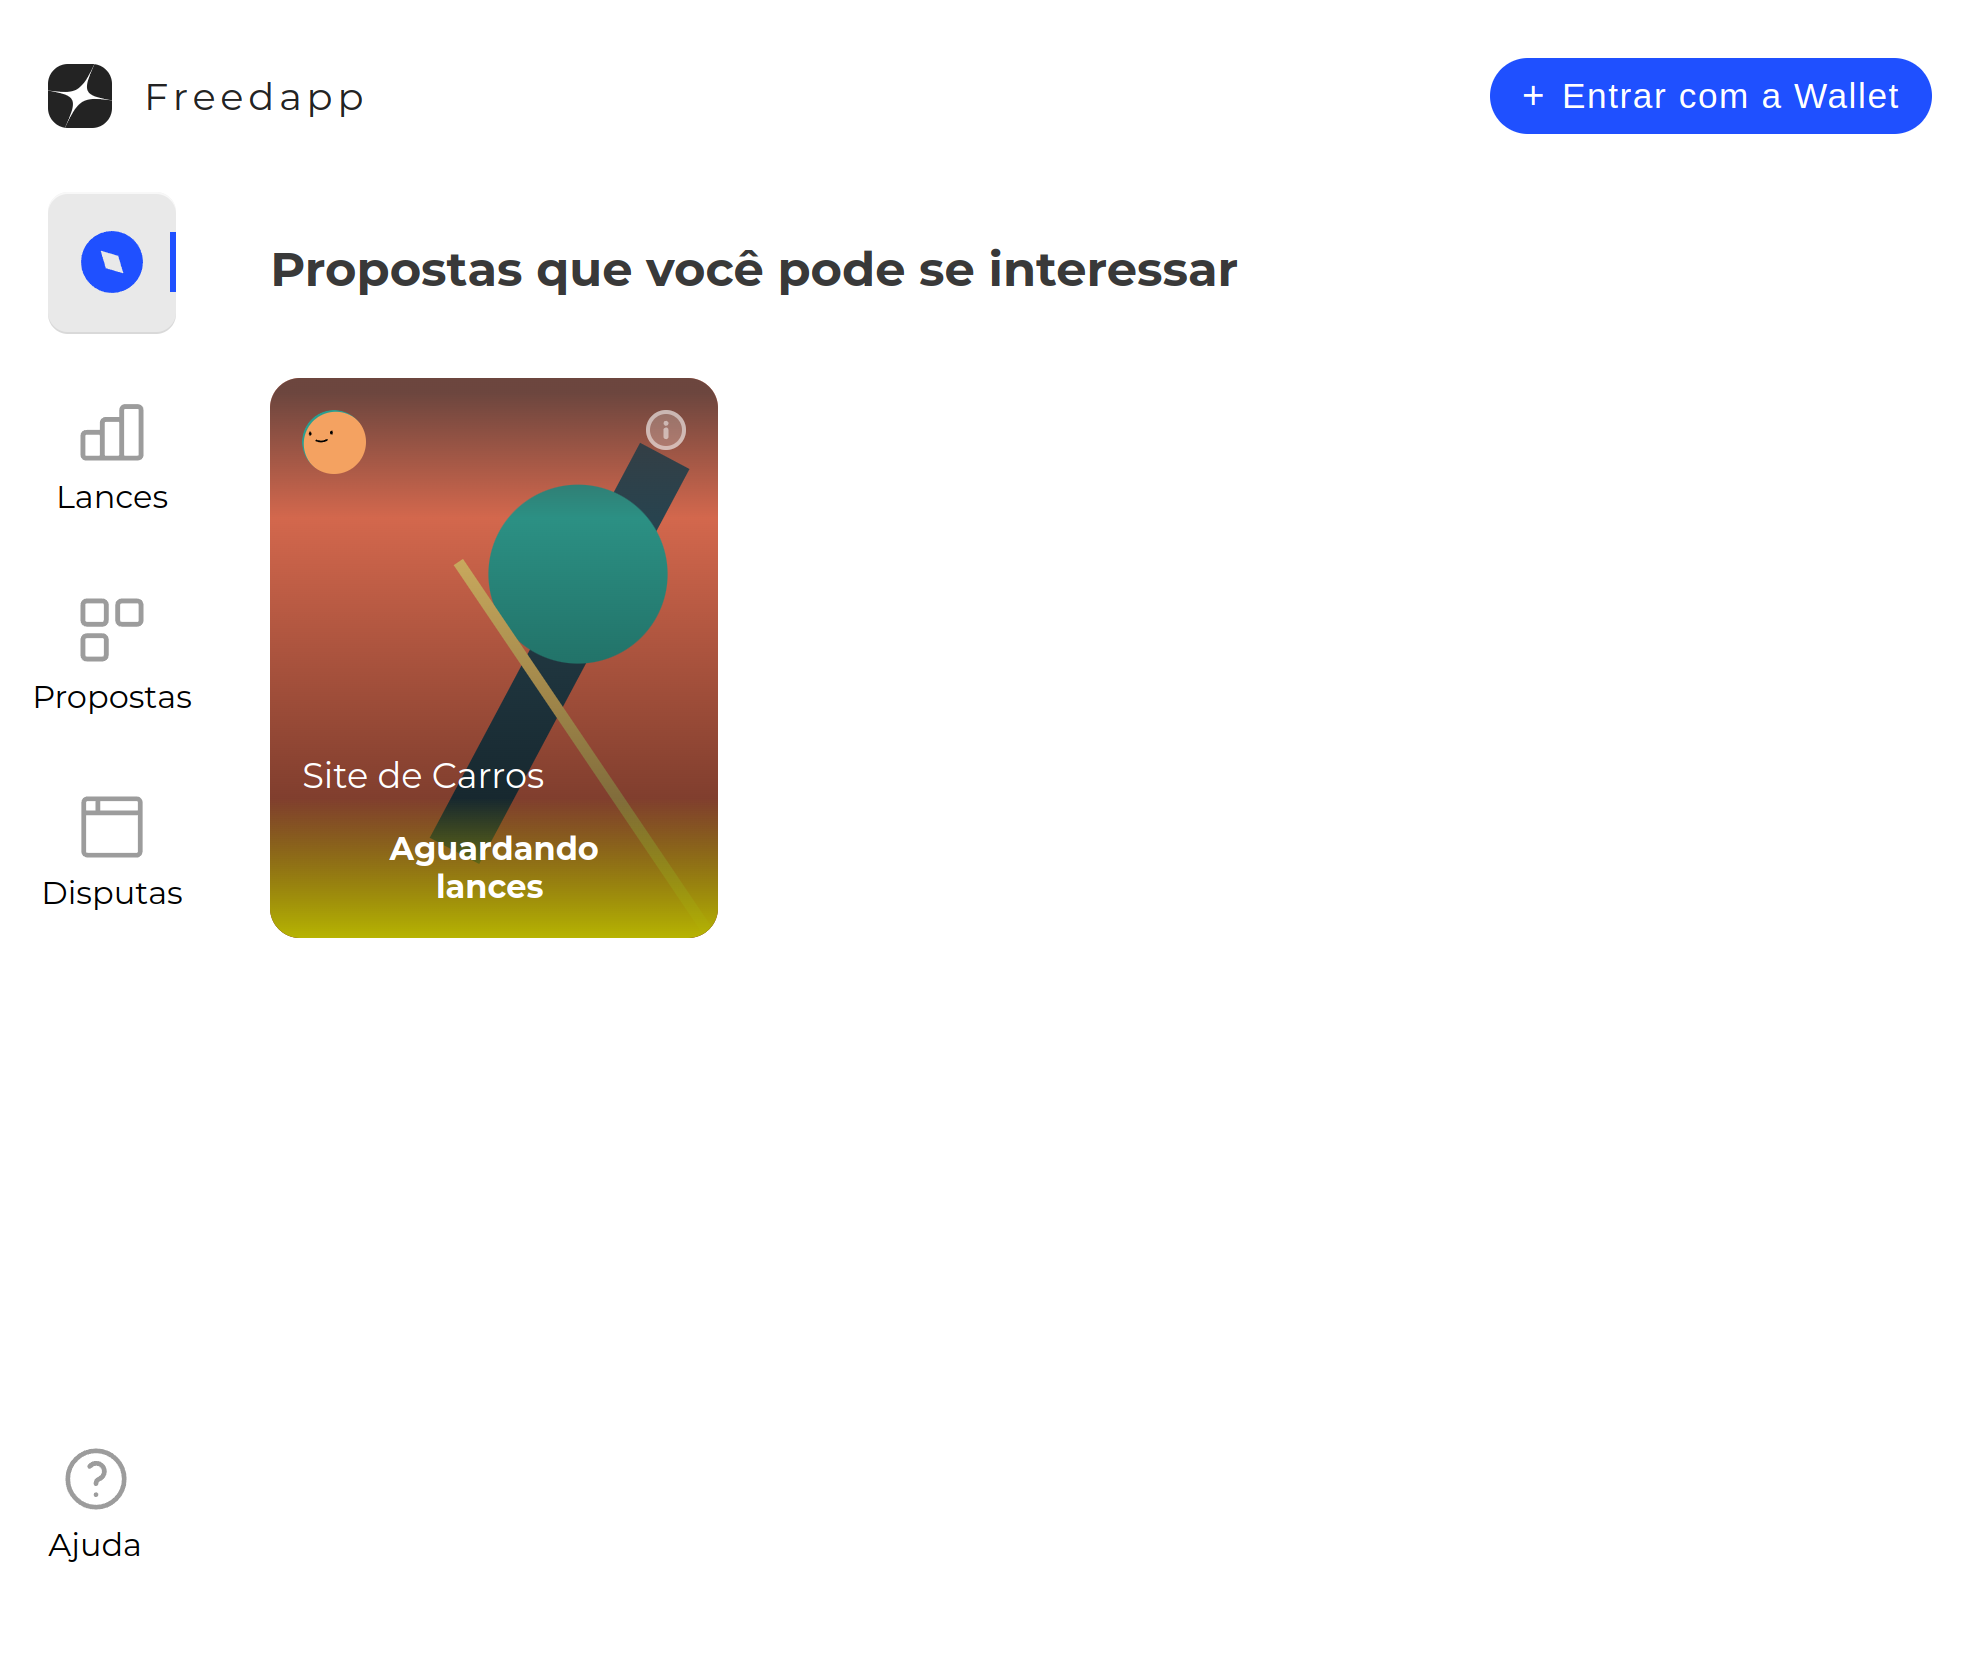
\includegraphics[width=450px]{src/images/app/home_page.png}
  \subcaption{Fonte: Autor }
  \label{fig:home_page_fig}
\end{figure}

Pode-se clicar nos itens da lista, redirecionando o usuário para uma página mais detalhada sobre a proposta. Além de, no canto da página, poder entrar com sua \textit{wallet} e conectar-se ao \textit{Metamask} para utilizar o \textit{Ethereum} como moeda para suas transações.

Em mais detalhes da proposta (figura \ref{fig:proposal_detail_page_state_waiting_bid_fig}), pode-se visualizar mais informações sobre a proposta. Ver seu nome, sua descrição, seu valor, a identificação do criador, a lista de lances que a proposta já recebeu com valor do lance, identificação do criador do lance e data de criação do lance e também a opção do usuário, caso queira, dar seu próprio lance na proposta. Além disso, pode-se visualizar o botão de ''Cancelar proposta'' caso você seja o criador daquela proposta.

\begin{figure}[h!]
  \centering
  \caption{Tela de detalhes de uma proposta}
  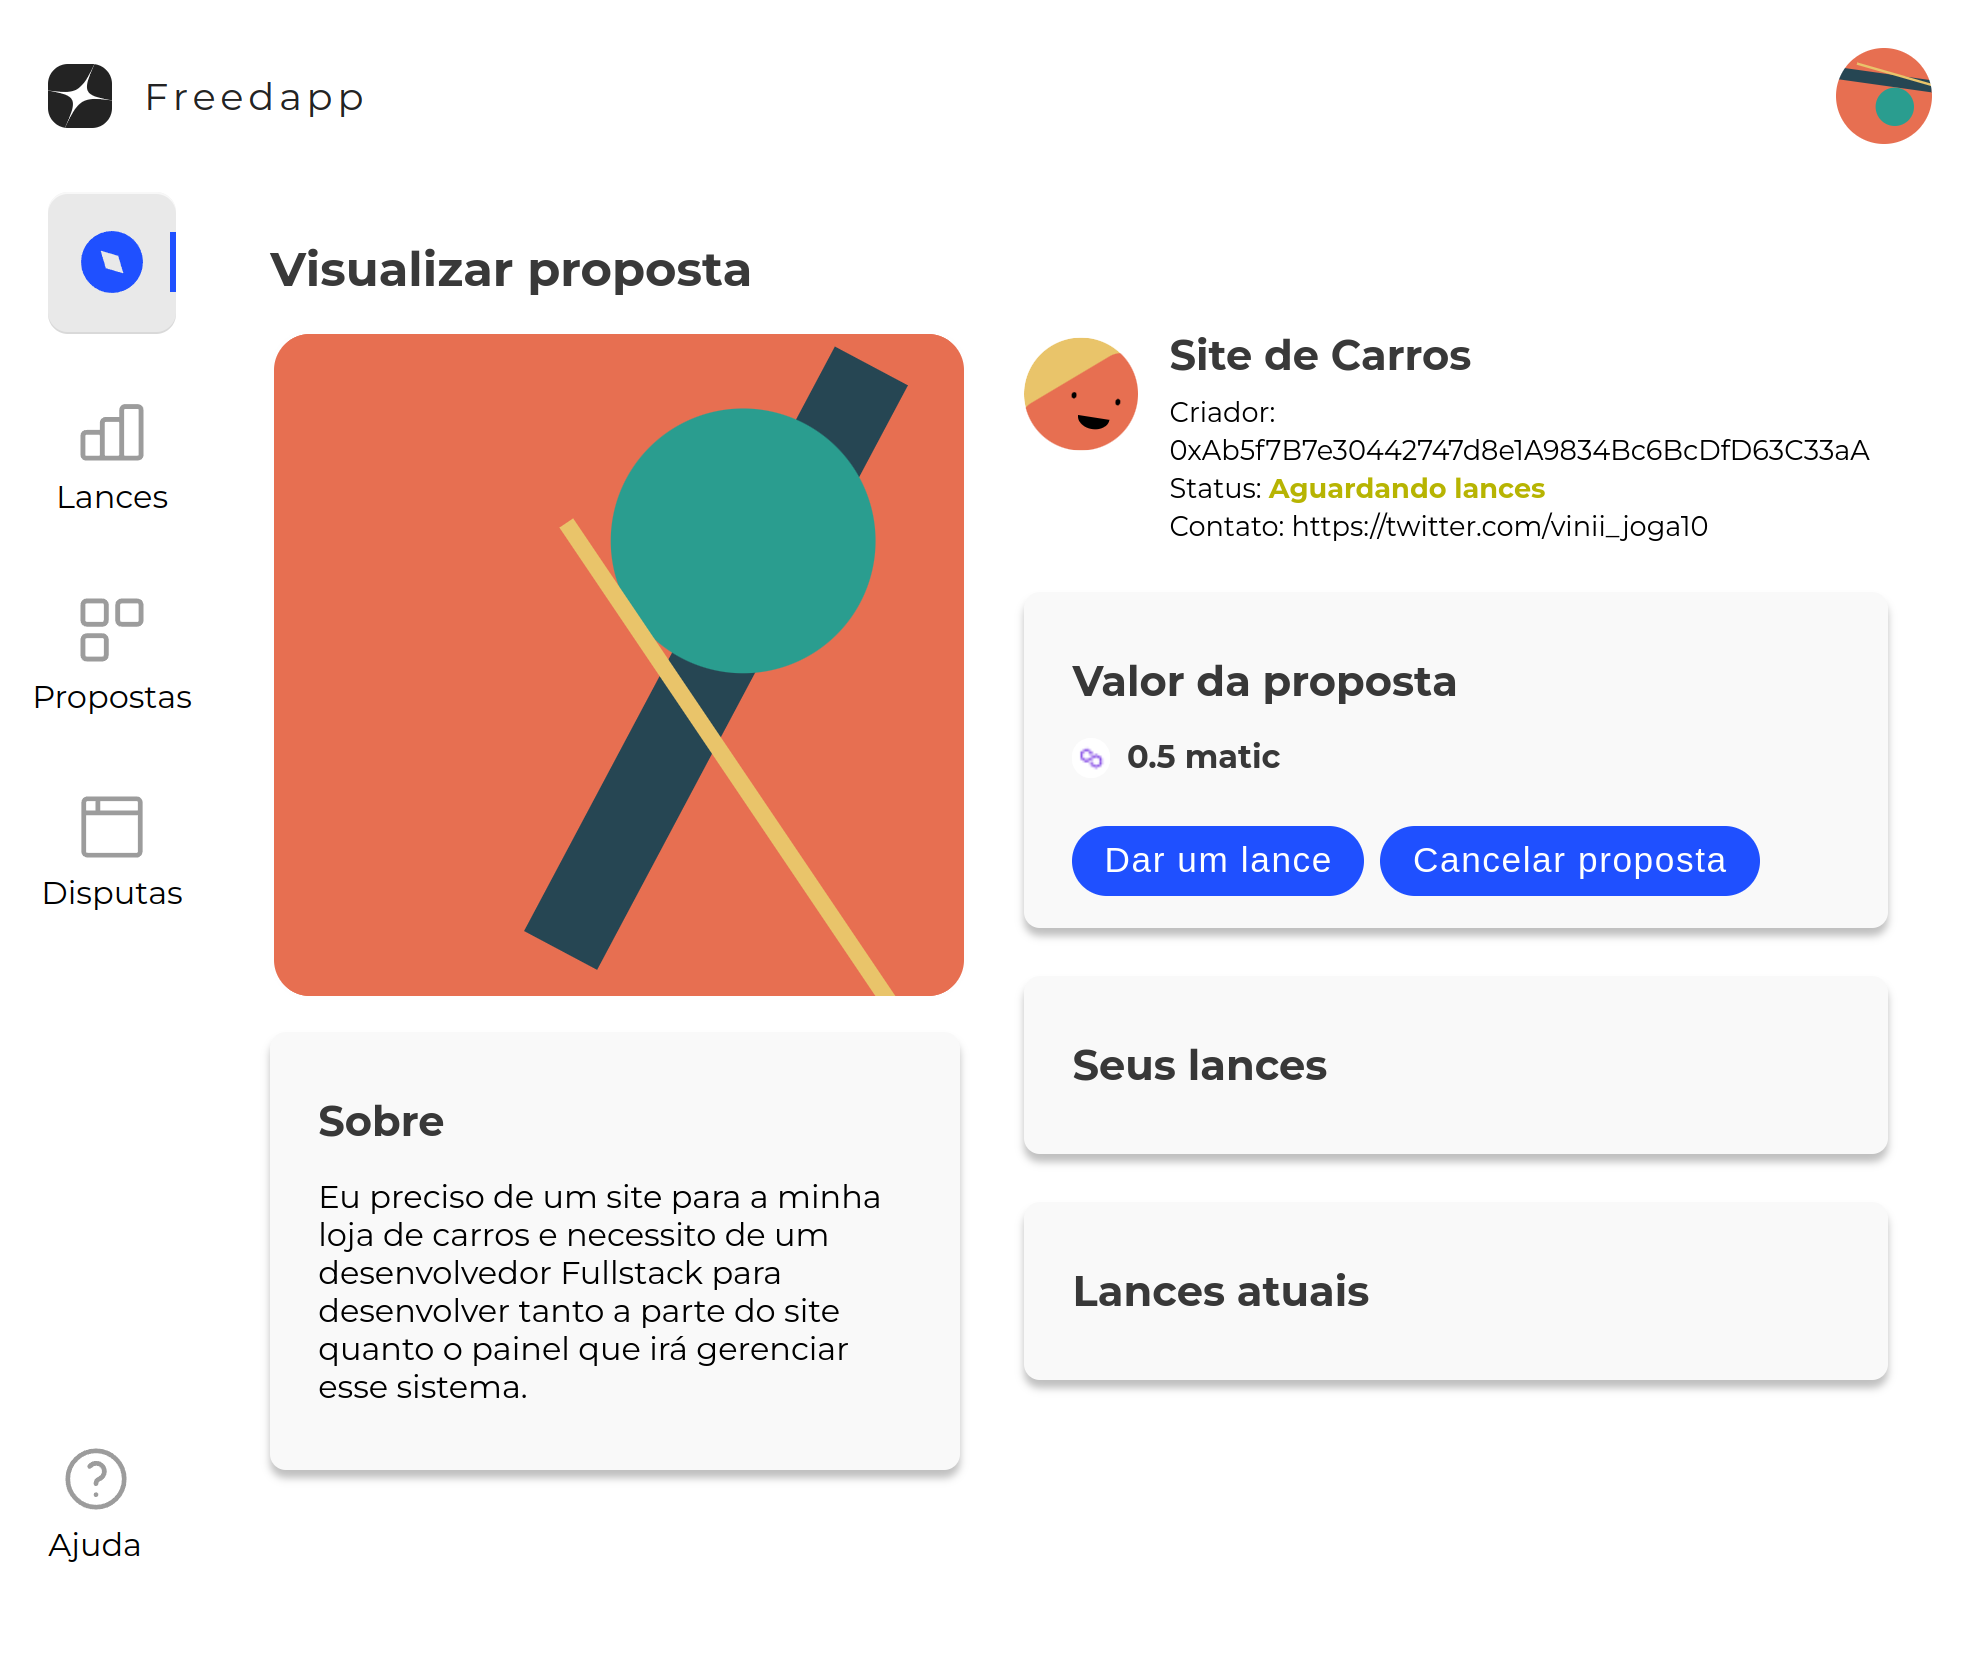
\includegraphics[width=450px]{src/images/app/proposal_detail_page_state_waiting_bid.png}
  \subcaption{Fonte: Autor }
  \label{fig:proposal_detail_page_state_waiting_bid_fig}
\end{figure}

Ao clicar em ''Dar um lance'' (figura \ref{fig:create_bid_modal_approval_fig}), é aberto automaticamente um popup do \textit{Metamask} para aprovar o lance sobre aquela proposta. O valor do lance é 5\% do valor da proposta, no qual é usado para filtrar pessoas realmente interessadas na proposta, e esse valor pode ser restituído se o usuário decidir cancelar o lance.

\clearpage

\begin{figure}[!h]
  \centering
  \caption{Modal do Metamask para aprovar a criação do lance}
  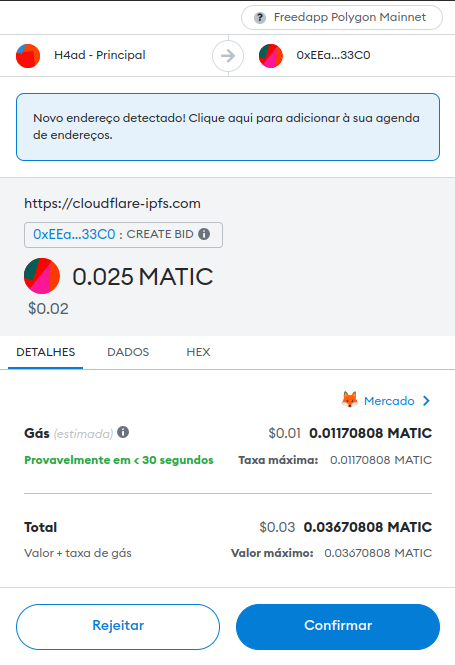
\includegraphics[height=450px]{src/images/app/create_bid_modal_approval.png}
  \subcaption{Fonte: Autor }
  \label{fig:create_bid_modal_approval_fig}
\end{figure}

Assim, ao confirmar, um novo componente gráfico aparecerá na tela (figura \ref{fig:proposal_detail_see_bid_fig}), caso o lance seja do usuário logado, irá ficar separado como "Seu lance", na qual, existe a possibilidade de visualizar a informação do seu lance ou remover o lance. Caso o lance não seja do usuário em questão, aparece como um item a mais na lista de lances daquela proposta. Ao retirar seu lance da proposta feito anteriormente, ele não pode ser mais selecionado pelo criador da proposta.

\clearpage

\begin{figure}[!h]
  \centering
  \caption{Visualizar um lance criado em aguardando lances}
  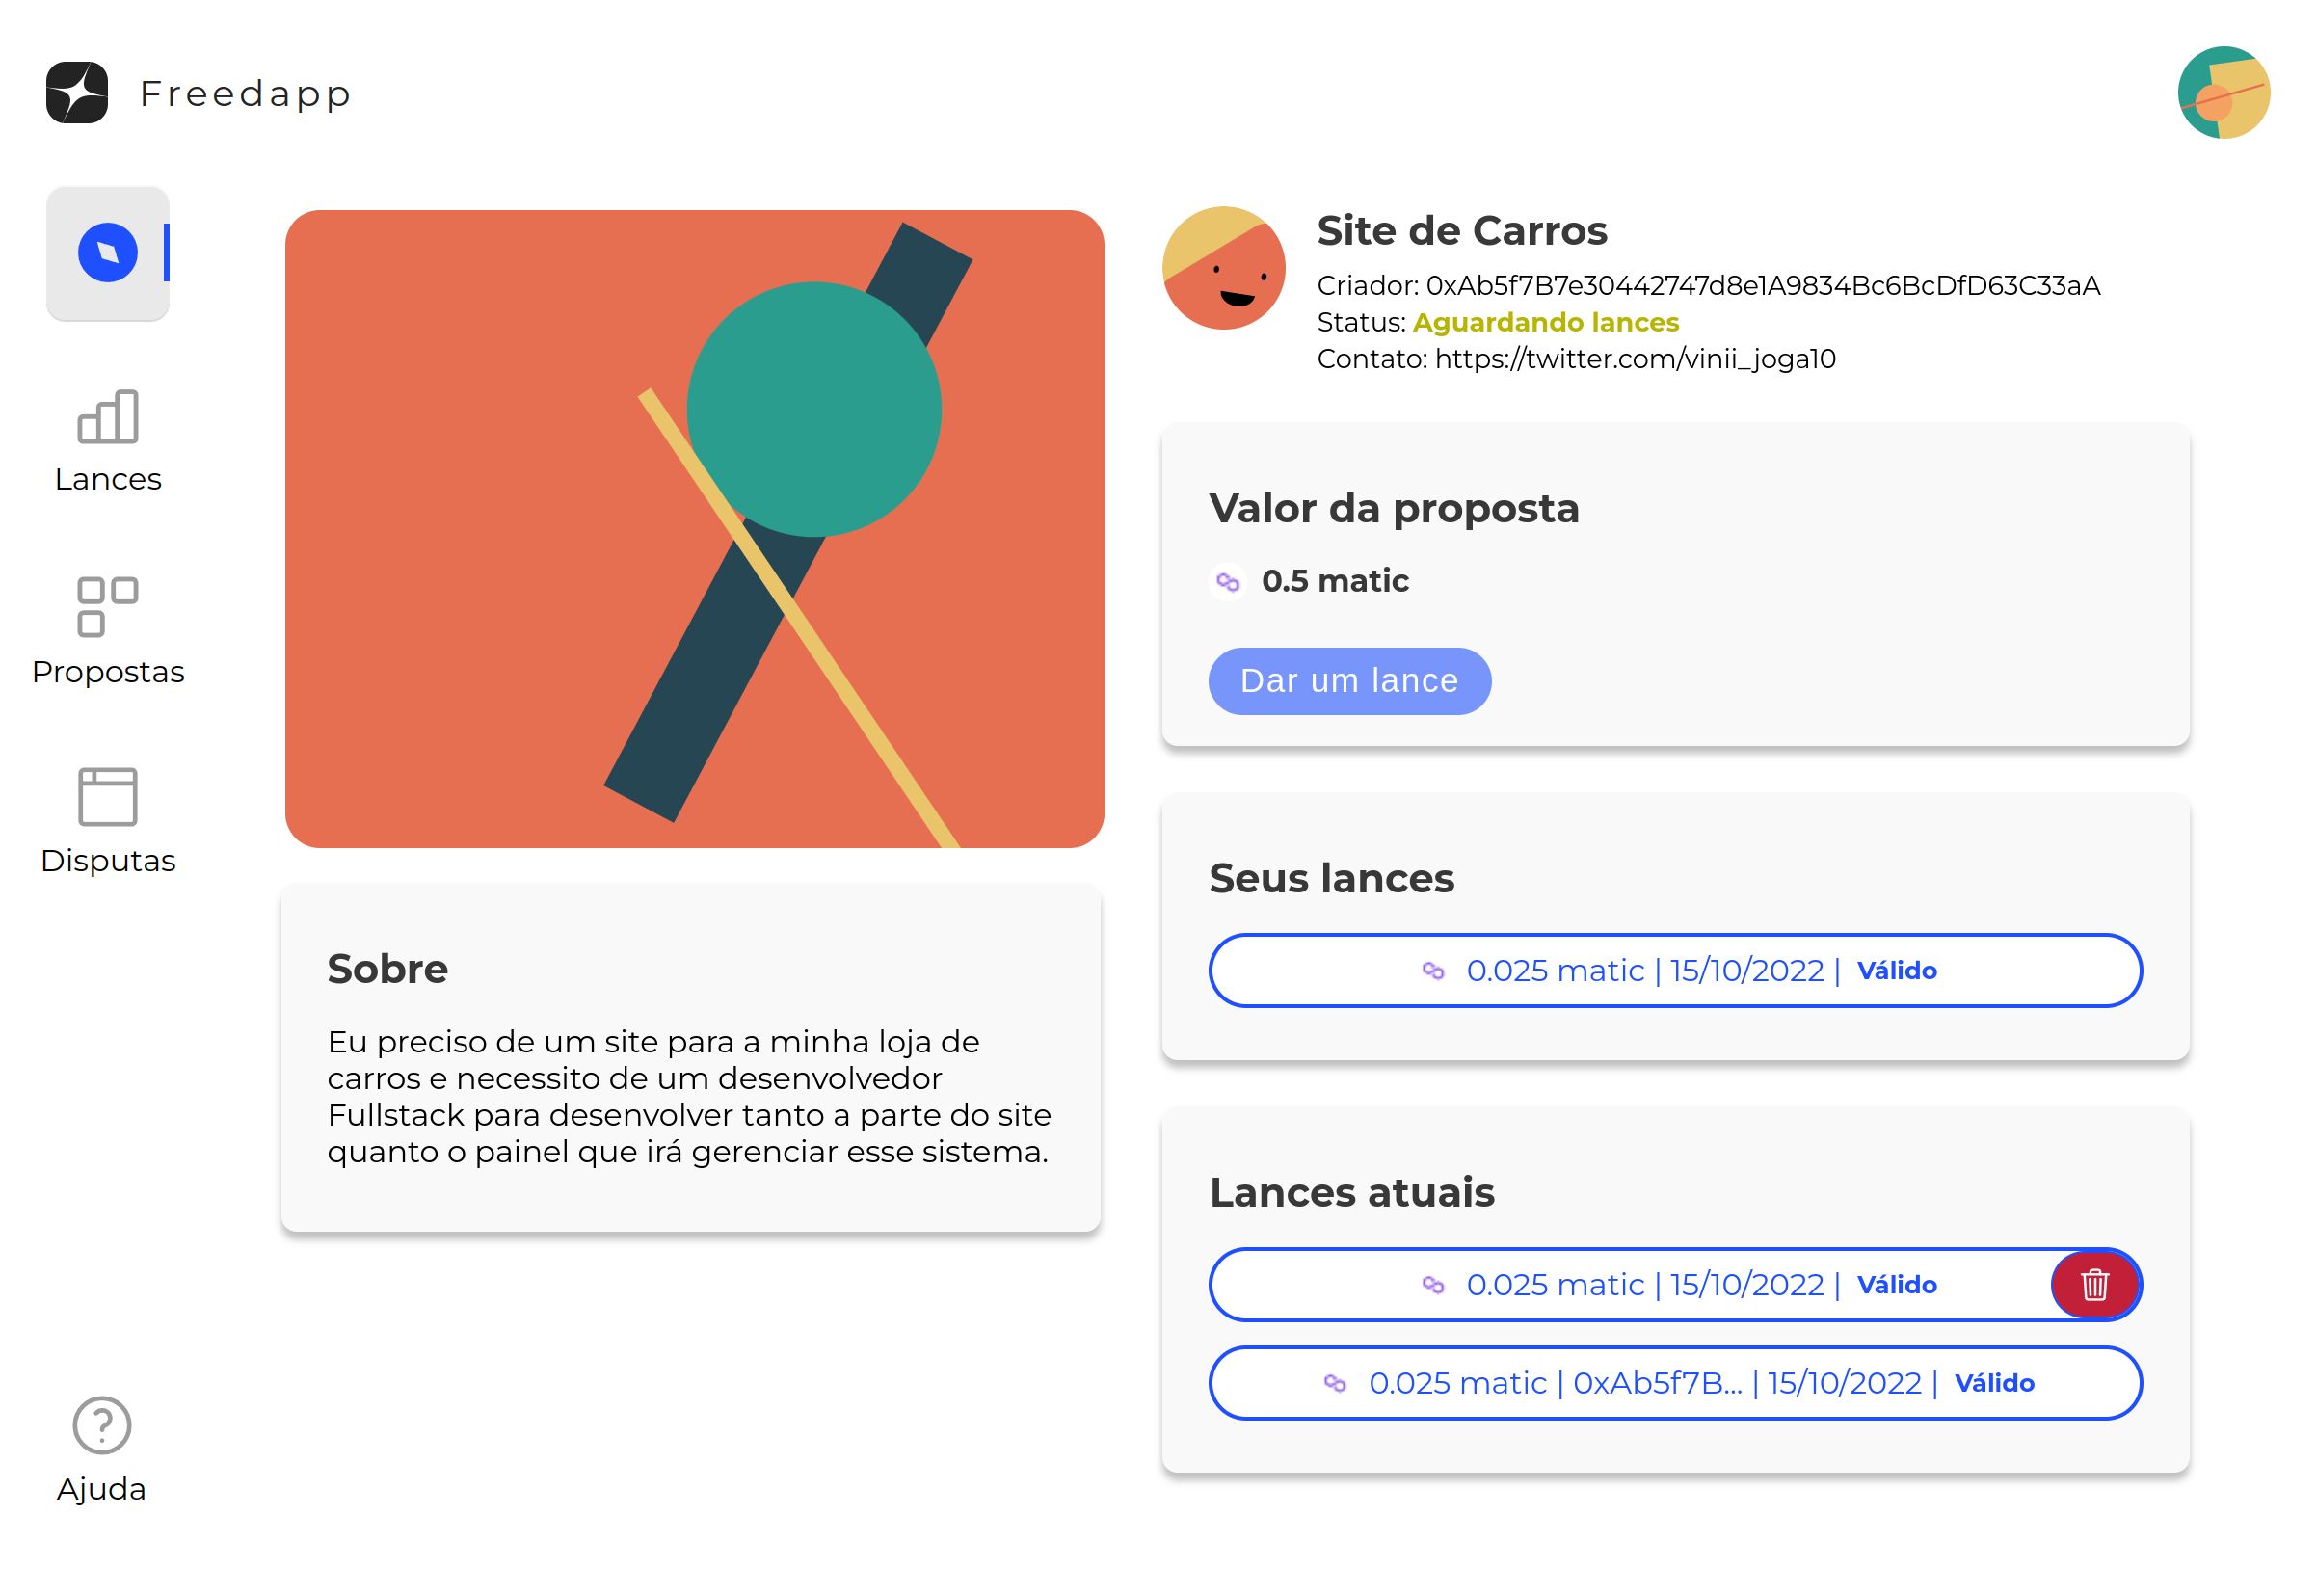
\includegraphics[width=450px]{src/images/app/proposal_detail_see_bid.png}
  \subcaption{Fonte: Autor }
  \label{fig:proposal_detail_see_bid_fig}
\end{figure}

Na página de lances (figura \ref{fig:bid_page_my_bids_fig}), pode-se ver a lista de itens dos lances do usuário logado com informações resumidas igual a tela de início porém com o detalhe do status do lance, caso o lance já tenha sido aceito pelo empregador, aparecerá ''Selecionado'', caso contrário irá continuar aparecendo ''Aguardando lance'' ou ''Rejeitado''. Quando o lance é rejeitado, o freelancer pode ir e recuperar o lance feito, recebendo de volta o valor pago durante a criação do lance.

\begin{figure}[!h]
  \centering
  \caption{Página de listagem de lances}
  
\includegraphics[width=400px]{src/images/app/bid_page_my_bids.png}
  \subcaption{Fonte: Autor }
  \label{fig:bid_page_my_bids_fig}
\end{figure}

Clicando em um lance ainda em progresso, o usuário será redirecionado para a página de detalhes da proposta, com informações da proposta e sua lista de lances e com as informações do seu lance e a possibilidade de remover o lance caso desejado.

Clicando em um lance já aceito, figura \ref{fig:proposal_details_creator_in_development_fig}, além de ver os detalhes da proposta, existe a opção de entrar em disputa com o empregador caso o freelancer achar necessário, ou enviar pagamento caso o freelancer já tenha finalizado o trabalho. Quanto ao botão de entrar em disputa, um novo fluxo é aberto, o qual será comentado mais a frente na parte de disputas.

\begin{figure}[!h]
  \centering
  \caption{Visualizar um lance criado em desenvolvimento}
  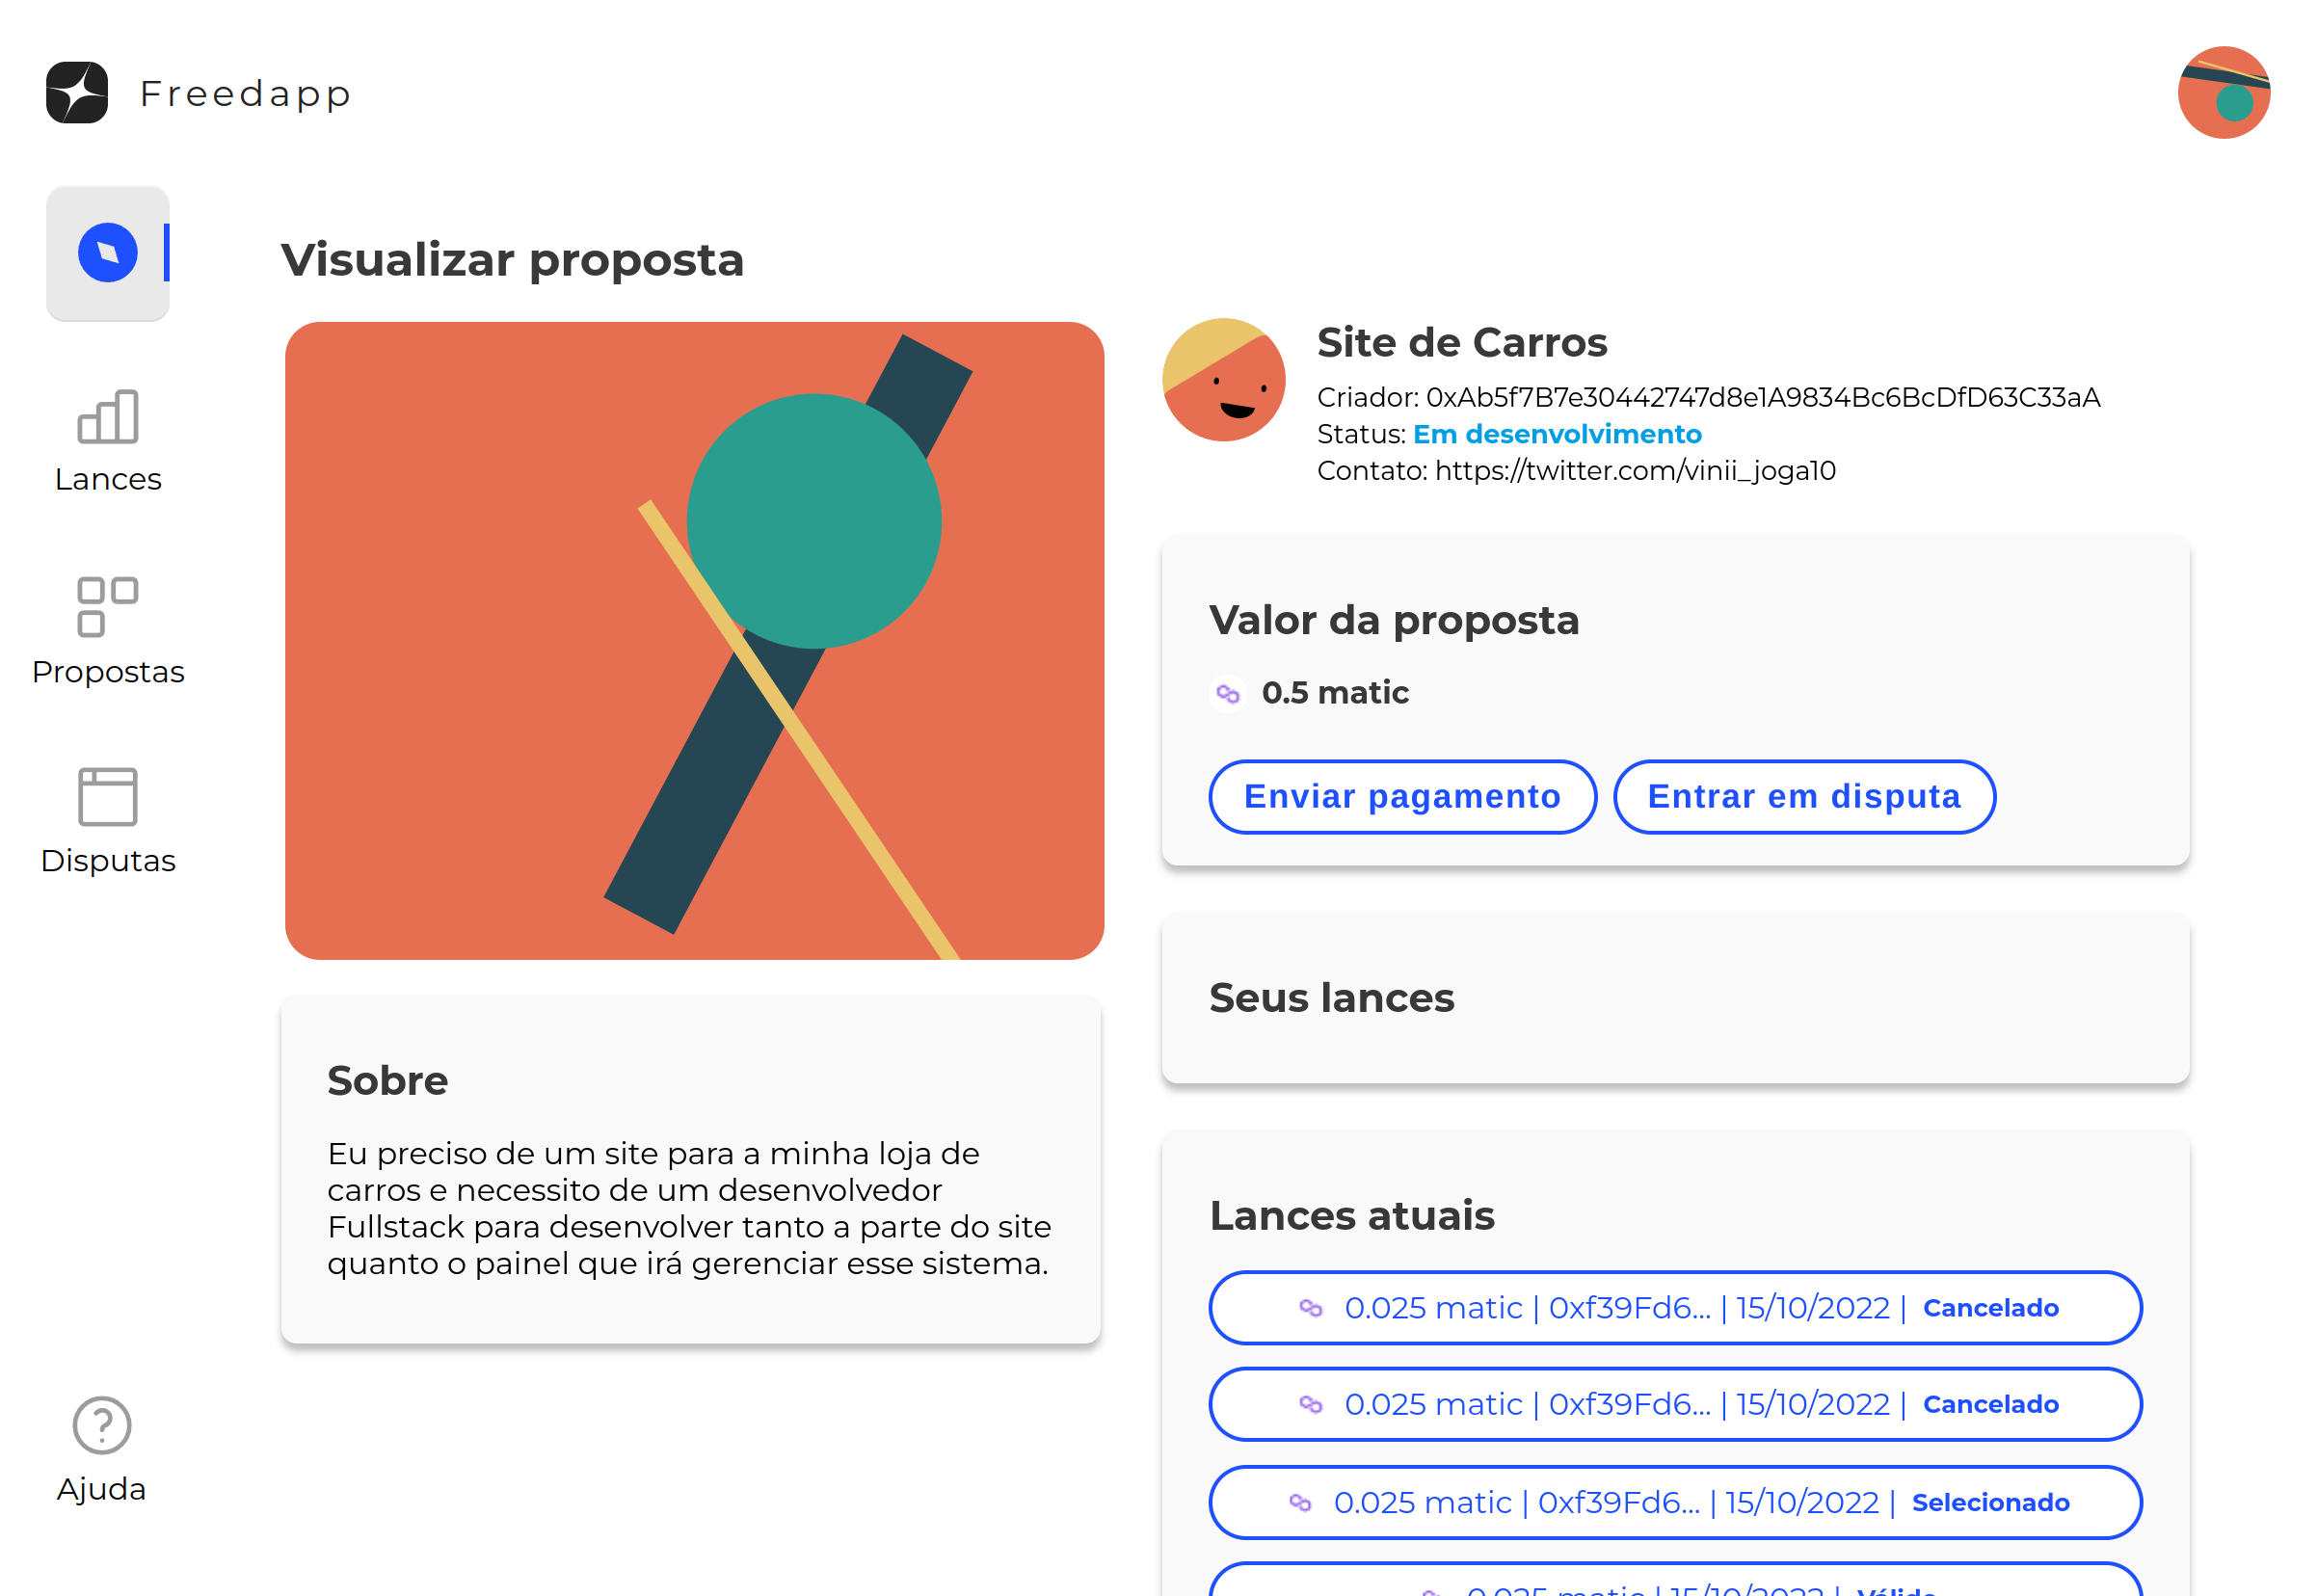
\includegraphics[width=400px]{src/images/app/proposal_details_creator_in_development.png}
  \subcaption{Fonte: Autor }
  \label{fig:proposal_details_creator_in_development_fig}
\end{figure}

Como dito anteriormente, o sistema não cobre a troca de mensagens entre o freelancer e o empregador, deixando opções para aplicativos e sistemas externos, como por exemplo, o e-mail.

Além de toda experiência como usuário freelancer, existe a possibilidade do usuário criar suas próprias propostas, pagando a outros usuário freelancers para executar seus projetos. Na página de proposta, os usuários logados podem ver suas propostas cadastradas com informações resumidas como nome e se a proposta já foi aceita, cancelada ou se continua em progresso, como demonstrado na figura \ref{fig:proposal_list_fig}. Ao clicar em um dos itens da lista de propostas, este é redirecionado para página de detalhes da proposta já descrita anteriormente. 

\begin{figure}[!h]
  \centering
  \caption{Lista da minhas propostas criadas}
  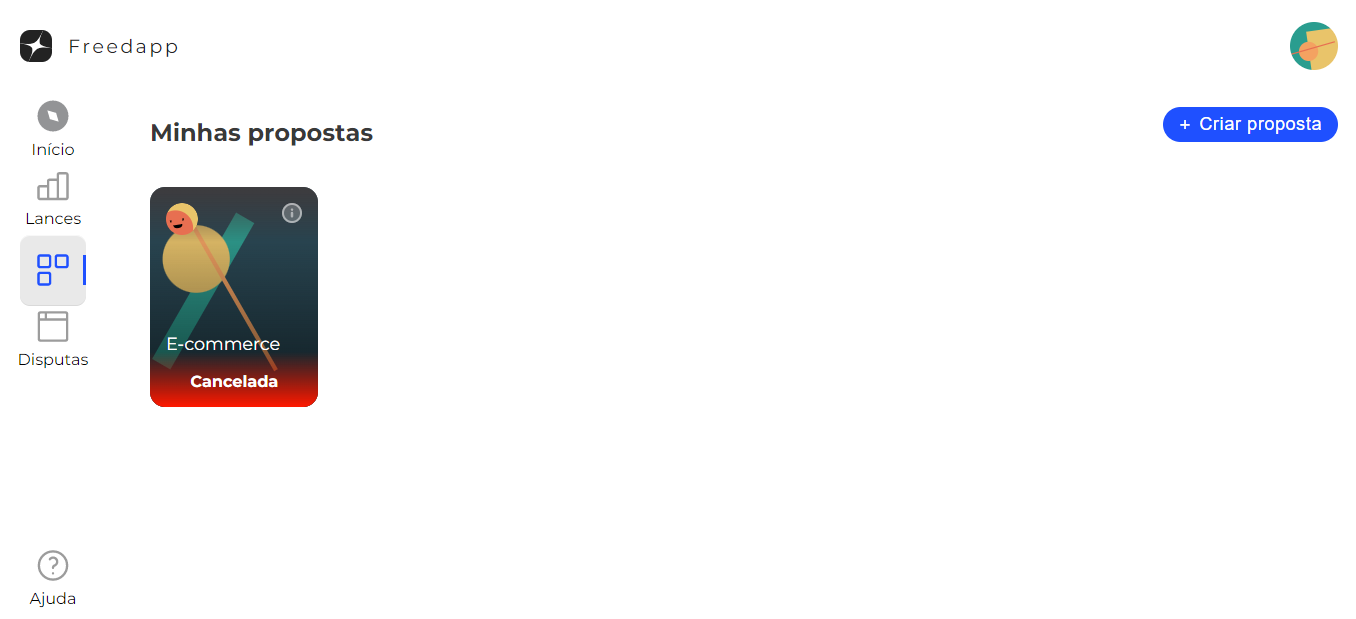
\includegraphics[width=400px]{src/images/app/proposal_list.PNG}
  \subcaption{Fonte: Autor }
  \label{fig:proposal_list_fig}
\end{figure}

Nesta página pode-se criar novas propostas, ao clicar em ''Criar proposta'' no canto superior direito, é aberta uma página de criação, demonstrada na figura \ref{fig:proposal_create_fig}, onde o usuário pode adicionar título/nome, descrição, valor, categoria e as informações de contato do empregador, estas são as informações necessárias para criação de uma proposta.

\begin{figure}[!h]
  \centering
  \caption{Formulário de criação de proposta}
  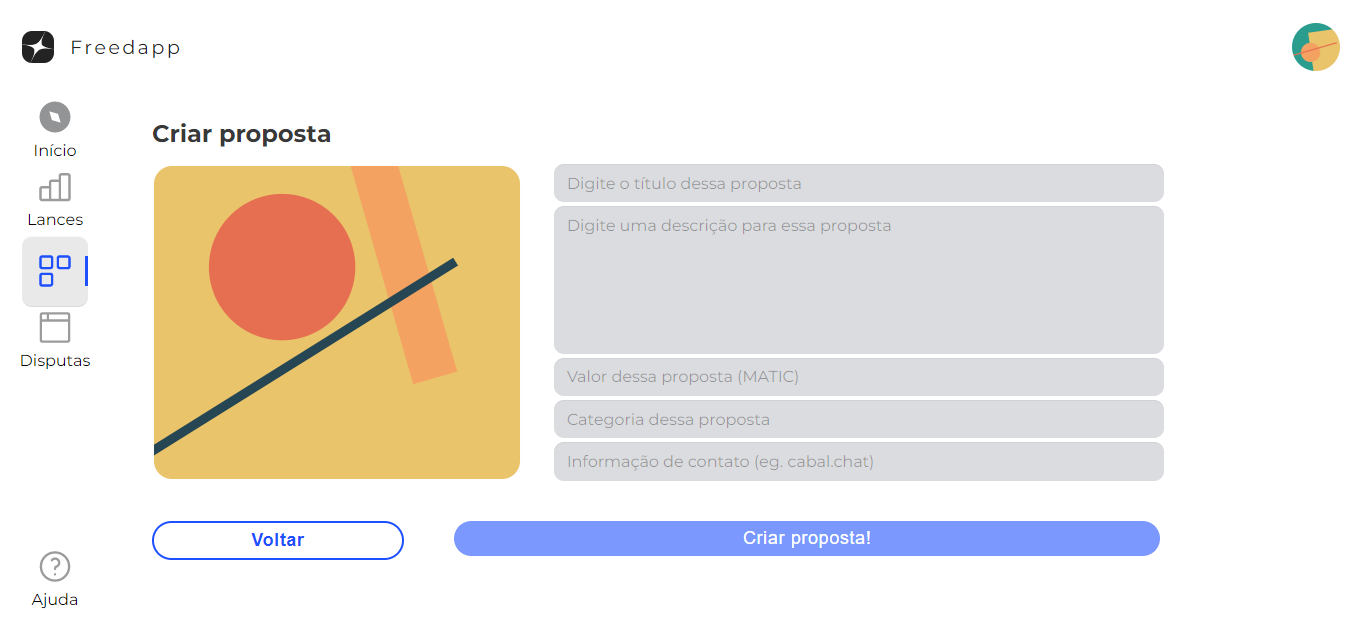
\includegraphics[width=400px]{src/images/app/proposal_create.PNG}
  \subcaption{Fonte: Autor }
  \label{fig:proposal_create_fig}
\end{figure}

A tela de disputas serve para a resolução de conflitos entre os freelancers e os empregados com relação a proposta e os lances. A página lista as disputas que aquele usuário logado participa ou participou, exibindo o nome da proposta e o status da disputa, exemplo na figura \ref{fig:dispute_list_fig}.

\begin{figure}[!h]
  \centering
  \caption{A lista de disputas do usuário}
  
\includegraphics[width=400px]{src/images/app/dispute_list.PNG}
  \subcaption{Fonte: Autor }
  \label{fig:dispute_list_fig}
\end{figure}

Os possíveis status da disputa são:
\begin{itemize}
    \item Escolher mediador
    \item Distribuir valores
    \item Disputa finalizada
\end{itemize}

A disputa inicialmente requer que ambos os lados escolham um mediador, digitando a identificação do mesmo. Para prosseguir para próxima etapa ambos devem escolher o mesmo mediador, portanto, se necessário, há a opção de entrar em contato por meios externos para coordenarem a escolha.

Após o mediador ser escolhido por ambos e acordado, o mediador analisa e pondera os lados, enquanto isso os usuários aguardam a resposta do mediador. Por fim, o mediador diz qual será a porcentagem de saldo distribuído, tanto para o freelancer quanto para o empregador, finalizando a disputa. O mediador ganha uma taxa de 5\% do valor total transacionado como incentivo para realizar seu trabalho de mediador. As figuras \ref{fig:dispute_mediator_list_fig} e \ref{fig:dispute_mediator_values_fig} mostram a visão do mediador.

\begin{figure}[!h]
  \centering
  \caption{As disputas na visão do mediador}
  
\includegraphics[width=400px]{src/images/app/dispute_mediator_list.PNG}
  \subcaption{Fonte: Autor }
  \label{fig:dispute_mediator_list_fig}
\end{figure}

\begin{figure}[!h]
  \centering
  \caption{O mediador distribuindo valores}
  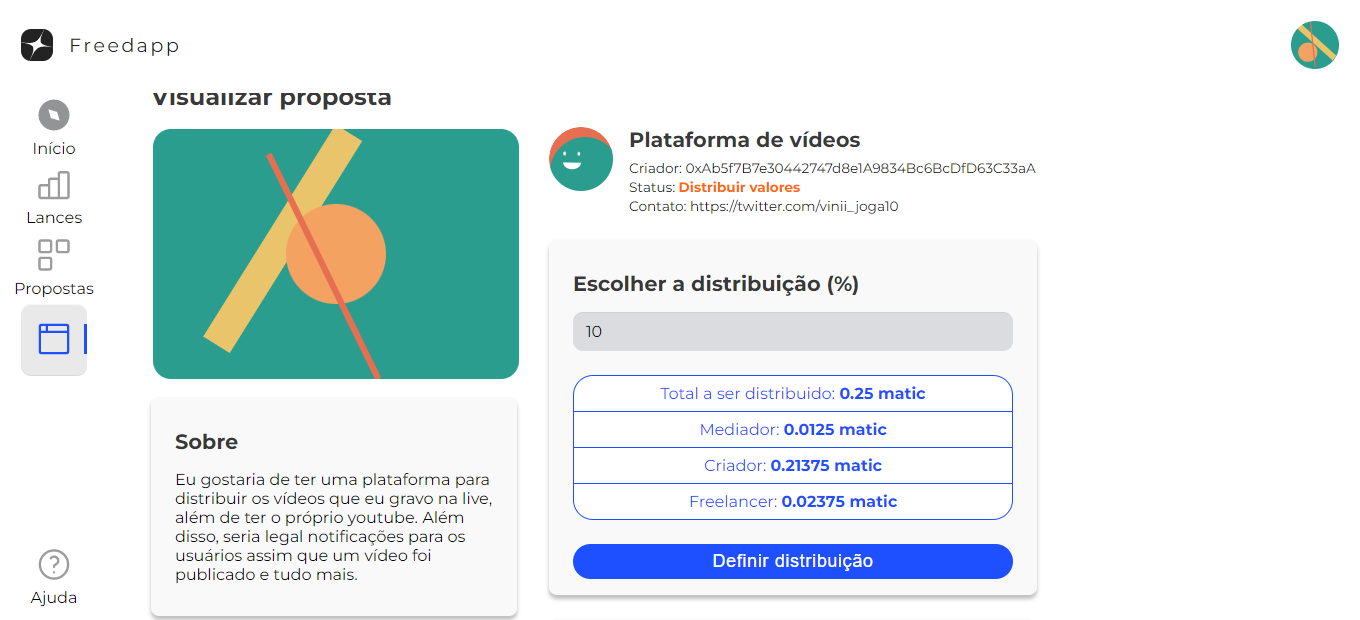
\includegraphics[width=400px]{src/images/app/dispute_mediator_values.PNG}
  \subcaption{Fonte: Autor }
  \label{fig:dispute_mediator_values_fig}
\end{figure}

Após concluída a distribuição de valores pelo mediator a disputa é finalizada e os valores do freelancer e o do empregador são automaticamente transferidos. Agora, após o processo de disputa, na lista de disputas do usuário, a proposta consta como ''Finalizada'' como mostrado na figura \ref{fig:dispute_finish_fig}.

\begin{figure}[!h]
  \centering
  \caption{Lista de disputas do usuário}
  
\includegraphics[width=400px]{src/images/app/dispute_finish.PNG}
  \subcaption{Fonte: Autor }
  \label{fig:dispute_finish_fig}
\end{figure}

Por fim, temos a tela de ajuda, que tem por objeto sanar as dúvidas dos usuários e mostrar como funciona o FreedApp, além de possuir tutoriais, como por exemplo ''Como instalar o MetaMask''.

\section{Smart Contracts}

Assim como no caso do site, os \textit{Smart Contracts} foram hospedados na rede de teste da \textit{Polygon} chamada \textit{Mumbai}, e assim como planejado no desenvolvimento, foi hospedado três contratos com os seguintes endereços:

\begin{itemize}
    \item Proposta: \textit{0x0672C724765Ca66BB9325881A7ACA1dfB3854137}
    \item Lances: \textit{0xEEa3e8974C2f631D4E0351F5f30997fD311633C0}
    \item Disputas: \textit{0x84262946Bc86229D12D0F17C5F60726E760Ef3Ff}
\end{itemize}

Os contratos não possuem uma representação visual assim como um site mas a seguir será mostrado um pouco do código usado, assim como, as técnicas que foi utilizado para evitar o problema de \textit{Reentrancy}.

\subsection{Propostas}

O contrato de propostas interliga outros contratos além de realizar as operações básicas de propostas, sendo assim, o principal da aplicação desenvolvida. O contrato de proposta foi dividido em três sub-contratos definidos pelas interfaces de \textit{IProposalBase}, \textit{IProposalPermission} e \textit{IProposalCore}, responsáveis por operações básicas, validação de permissão e as operações principais, respectivamente.

A seguir, na figura \ref{fig:proposal_core_contract_fig}, alguns dos métodos disponíveis na interface do \textit{IProposalCore}. Pode-se observar diversos métodos com o prefixo ''\textit{on}'' como \textit{onBidderSelected} e \textit{onCreateDispute}. Esses métodos são usados para a comunicação entre outros contratos, sendo mais específico, para a comunicação do contrato de Lances e Disputas, para que o contrato de proposta seja atualizado quando, por exemplo, um lance for selecionado ou uma disputa for criada.

\begin{figure}[!h]
  \centering
  \caption{Interface do Contrato Core de Proposta}
  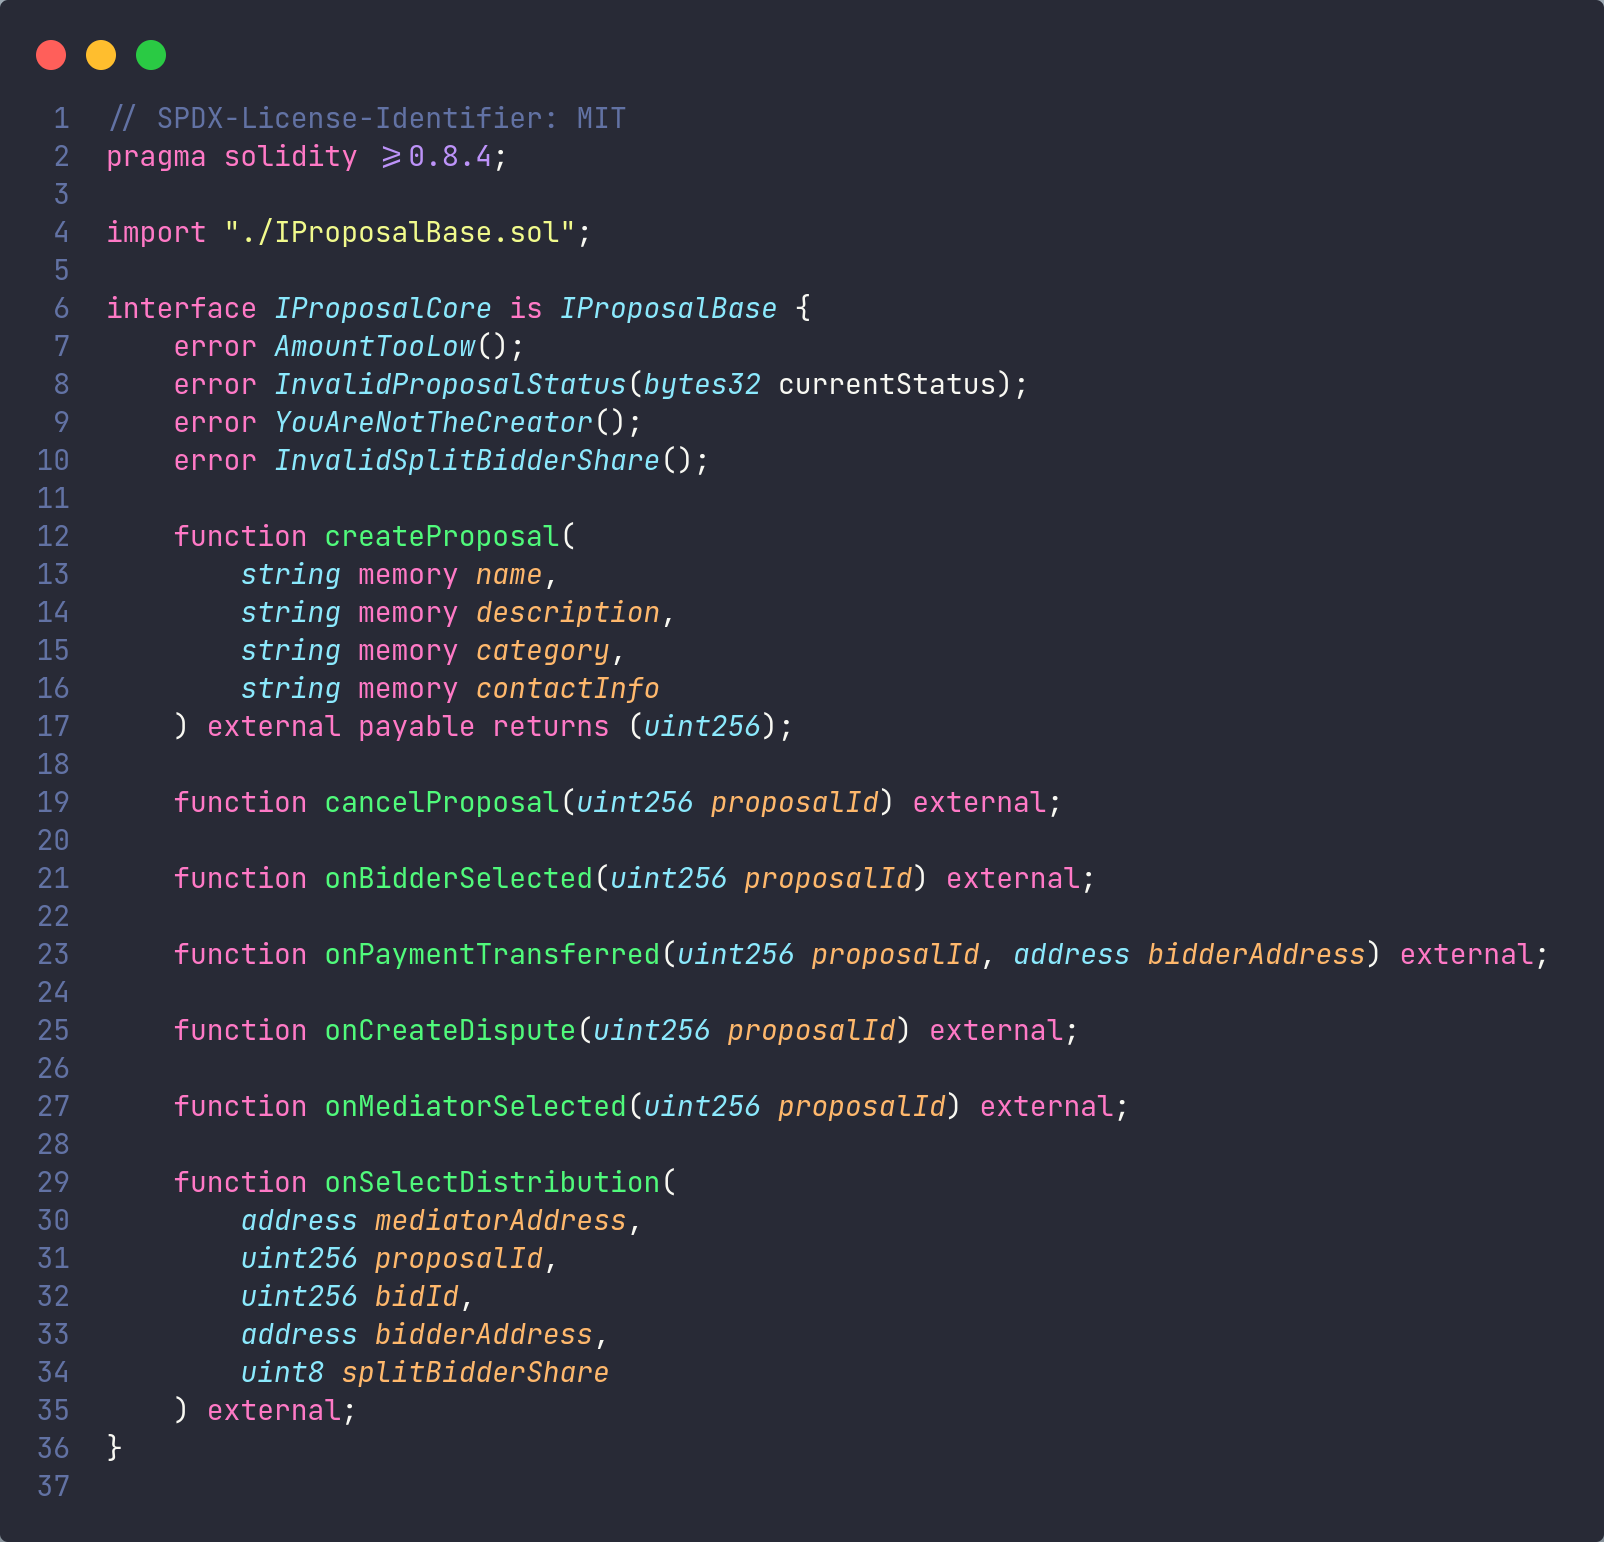
\includegraphics[width=320px]{src/images/contracts/proposal_core_contract.png}
  \subcaption{Fonte: Autor }
  \label{fig:proposal_core_contract_fig}
\end{figure}

Além dessa interface, há mais uma para representar as operações mais básicas de uma proposta, conforme mostrado na figura \ref{fig:proposal_base_contract_fig}. É interessante notar nos métodos como não há uma forma de retornar uma lista de propostas. Isso é pensado de forma proposital, e como descrito no desenvolvimento, é uma estratégia para economizar \textit{Gas} e reduzir custos da rede.

\begin{figure}[!h]
  \centering
  \caption{Interface do Contrato Base de Proposta}
  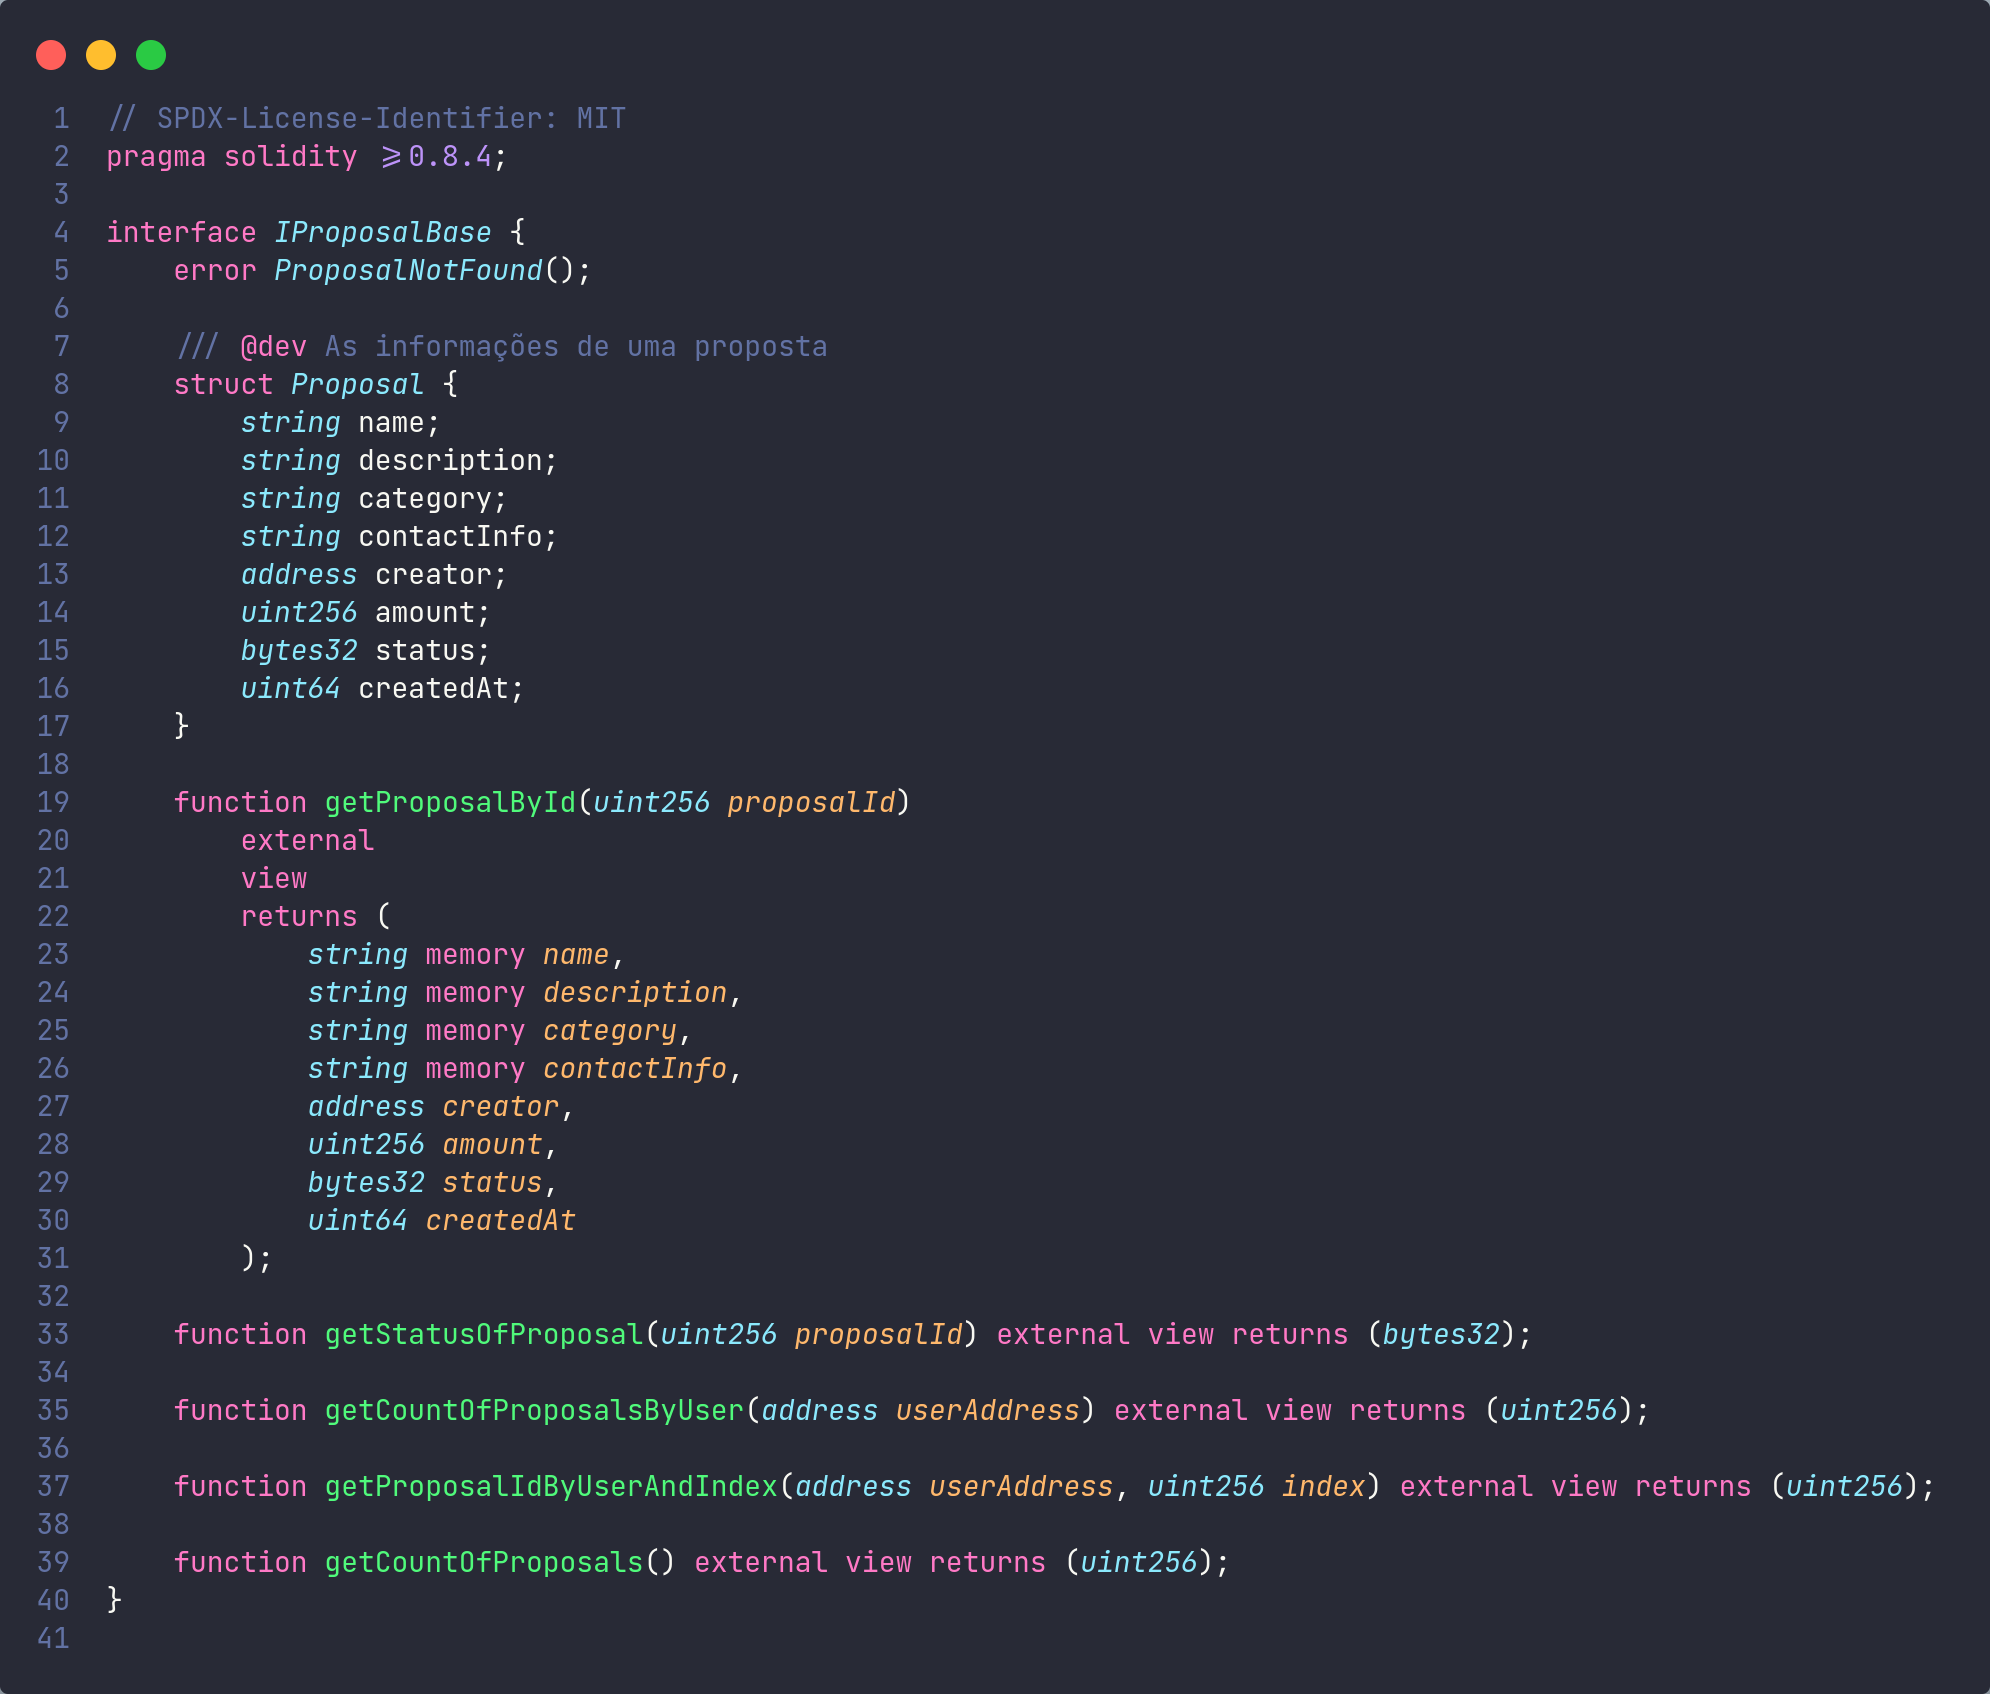
\includegraphics[width=320px]{src/images/contracts/proposal_base_contract.png}
  \subcaption{Fonte: Autor }
  \label{fig:proposal_base_contract_fig}
\end{figure}

Para que o usuário possa listar as propostas criadas no contrato, é necessário realizar duas operações básicas: \textit{getCountOfProposals} para saber quantas propostas existem e depois chamar o método \textit{getProposalById} para obter as informações da proposta. 

A identificação da proposta é incremental e começa em 1, dessa forma, se a contagem retornar 10, pode-se presumir com segurança que poderá obter as propostas com os \textit{IDs} de 1 a 10. Caso o usuário passe a identificação de uma proposta que não exista, é lançado um erro para alertar que não foi encontrado.

E por fim, para que o contrato de proposta saiba se deve ou não aceitar executar um método que é protegido para ser executado apenas pelo contrato de Lances ou Disputas, é usado a interface mostrado na figura \ref{fig:proposal_permission_contract_fig}.

\begin{figure}[!h]
  \centering
  \caption{Interface do Contrato Permission de Proposta}
  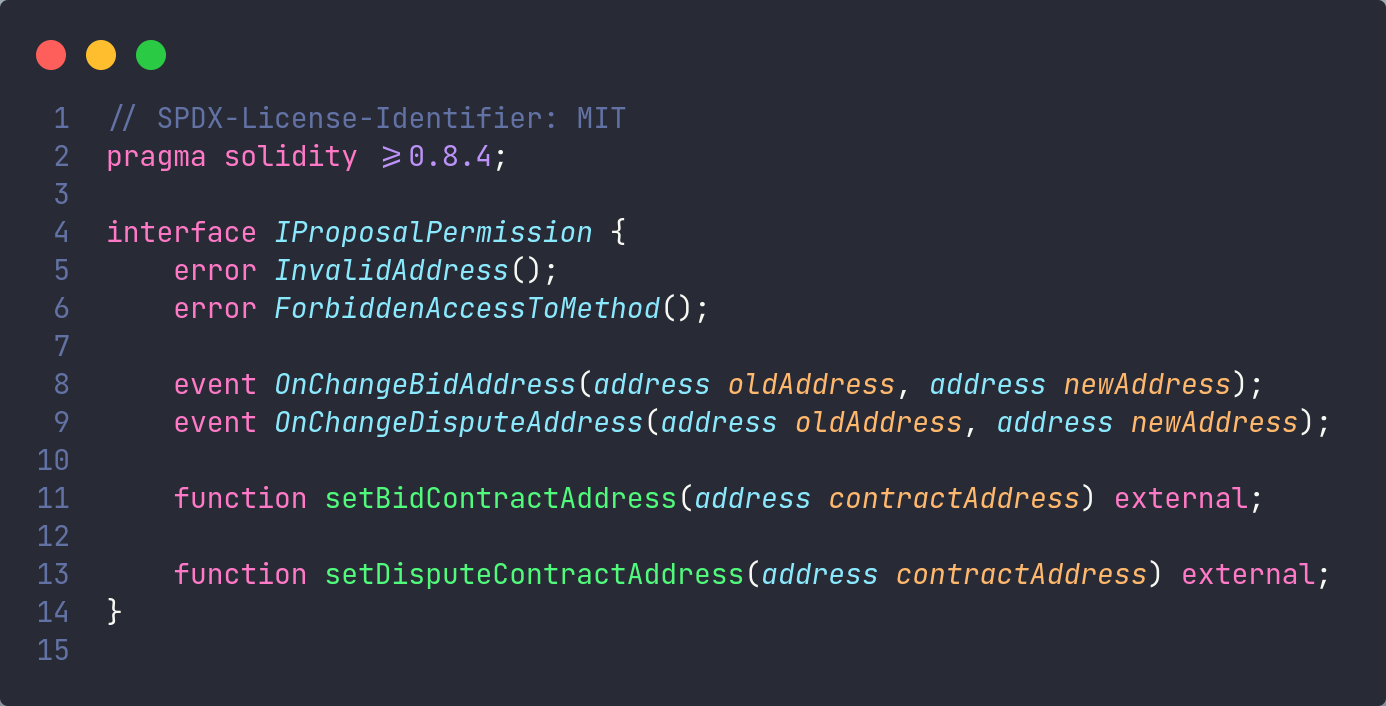
\includegraphics[width=320px]{src/images/contracts/proposal_permission_contract.png}
  \subcaption{Fonte: Autor }
  \label{fig:proposal_permission_contract_fig}
\end{figure}

Na figura \ref{fig:proposal_permission_contract_fig}, pode-se notar dois métodos no qual podem ser usados para especificar o endereço dos contratos de Lance e Disputa, dessa forma, quando o método for executado, bastaria checar se quem está executando bate com o endereço salvo no contrato de proposta.

Até esse ponto, o que foi mostrado é apenas o que foi exposto para o site consumir, quanto a sua implementação interna, será mostrado alguns trechos principais. Para começar, para solucionar o problema de \textit{Reentrancy}, o método de pagamento foi escrito como mostra a figura \ref{fig:proposal_core_on_payment_transferred_fig}.

\begin{figure}[!h]
  \centering
  \caption{Trecho de código do método onPaymentTransferred}
  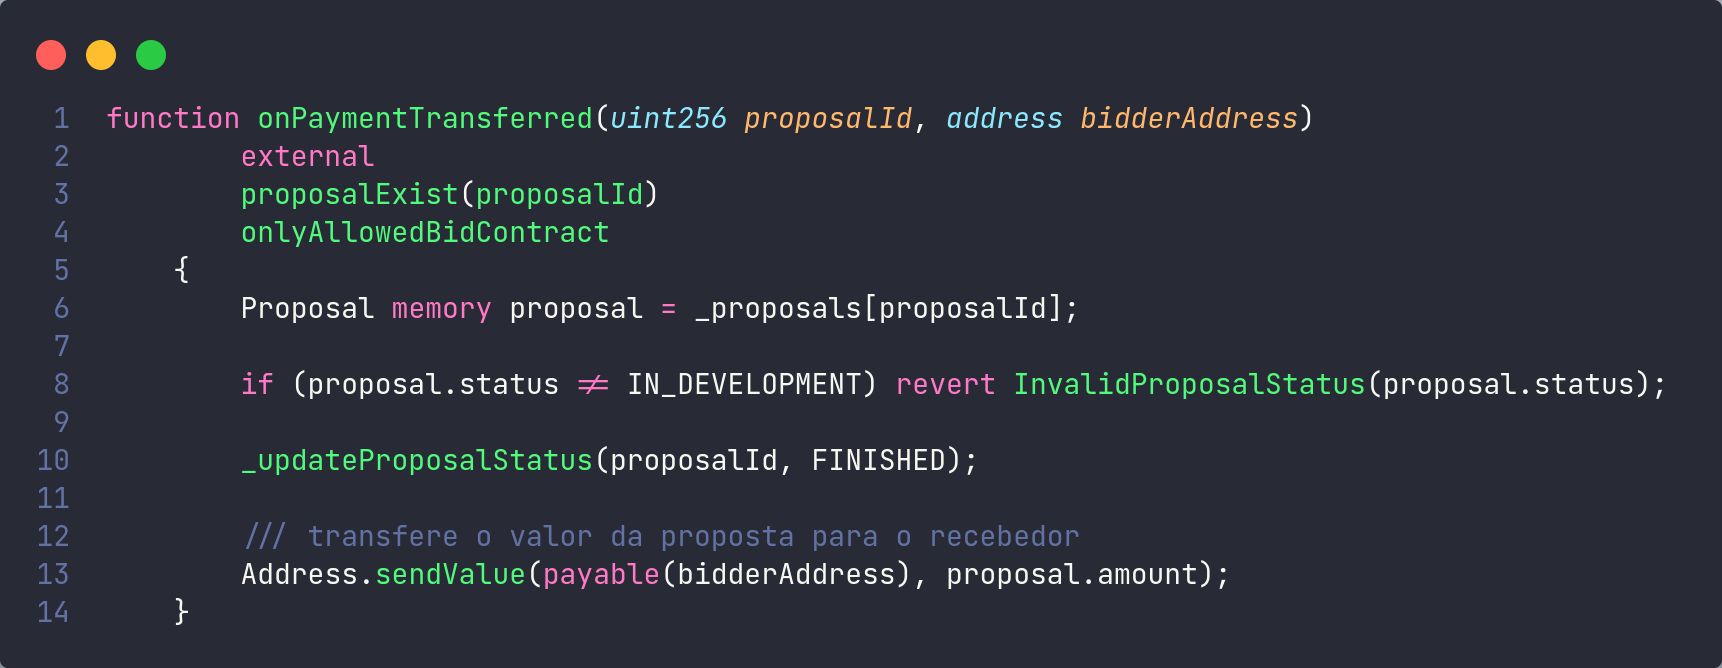
\includegraphics[width=350px]{src/images/contracts/proposal_core_on_payment_transferred.png}
  \subcaption{Fonte: Autor }
  \label{fig:proposal_core_on_payment_transferred_fig}
\end{figure}

Pode-se observar na linha 8 da figura \ref{fig:proposal_core_on_payment_transferred_fig}, a verificação do \textit{status} da proposta, só passará daquela verificação se o \textit{status} for igual \textit{IN\_DEVELOPMENT}, que significa que está em desenvolvimento. Após passar na verificação, imediatamente é chamado a função \textit{\_updateProposalStatus} que irá atualizar o \textit{status} da proposta para \textit{FINISHED}.

Dessa forma, esse método não poderá ser chamado novamente sem lançar o erro de \textit{InvalidProposalStatus}. Assim, o contrato é protegido de pessoas má intencionadas que buscam falhas para roubar todo o dinheiro do contrato.

Por fim, como medidas de segurança adicionais, o \textit{Solidity} possui a funcionalidade chamada \textit{Modifiers}, onde é criado uma função para validar se deve ou não executar o método em questão. Na função de \textit{onPaymentTransferred}, há dois \textit{Modifiers}: \textit{proposalExist} para checar se a proposta existe e \textit{onlyAllowedBidContract} que assegura que esse método só execute caso quem esteja chamando ele seja o contrato de Lances.

\subsection{Lances}

Após o contrato de propostas, o contrato de lances será um dos mais usados e ele foi dividido, assim como o contrato de propostas, em três sub-contratos chamados de \textit{IBidCore}, \textit{IBidBase} e o contrato \textit{BidProposal}, responsáveis por operações básicas, interação entre lance-proposta e ações principais, respectivamente.

A seguir, na figura \ref{fig:bid_core_contract_fig} pode-se observar alguns dos métodos disponíveis na interface de \textit{IBidCore}.

\begin{figure}[!h]
  \centering
  \caption{Interface do contrato IBidCore de Lances}
  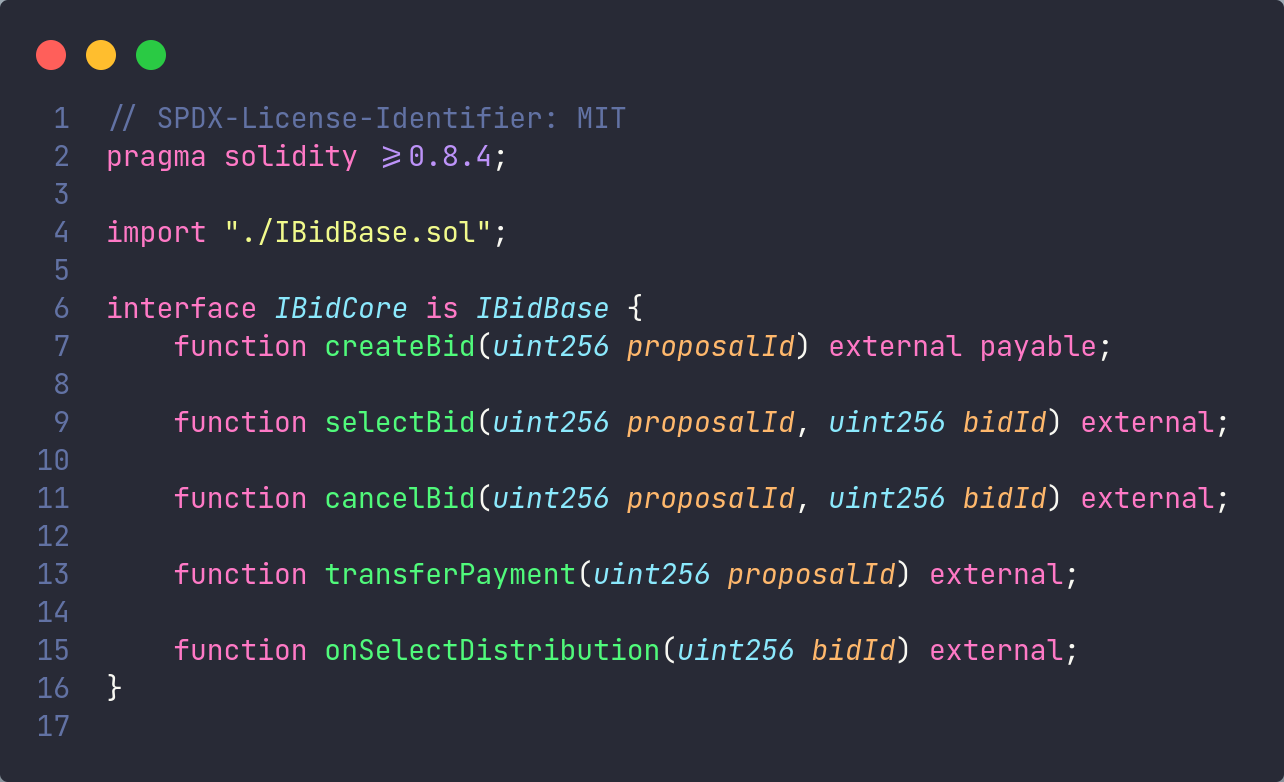
\includegraphics[width=320px]{src/images/contracts/bid_core.png}
  \subcaption{Fonte: Autor }
  \label{fig:bid_core_contract_fig}
\end{figure}

Assim como em propostas, o contrato de \textit{IBidCore} possui alguns métodos com a intenção de ser usado por outros contratos, no caso, o \textit{onSelectDistribution} tem a intenção de ser usado pelo contrato de disputas.

Após isso, como é ilustrado na figura \ref{fig:bid_base_contract_fig}, a interface \textit{IBidBase} do contrato base de lances.

\begin{figure}[!h]
  \centering
  \caption{Interface do contrato Base de Lances}
  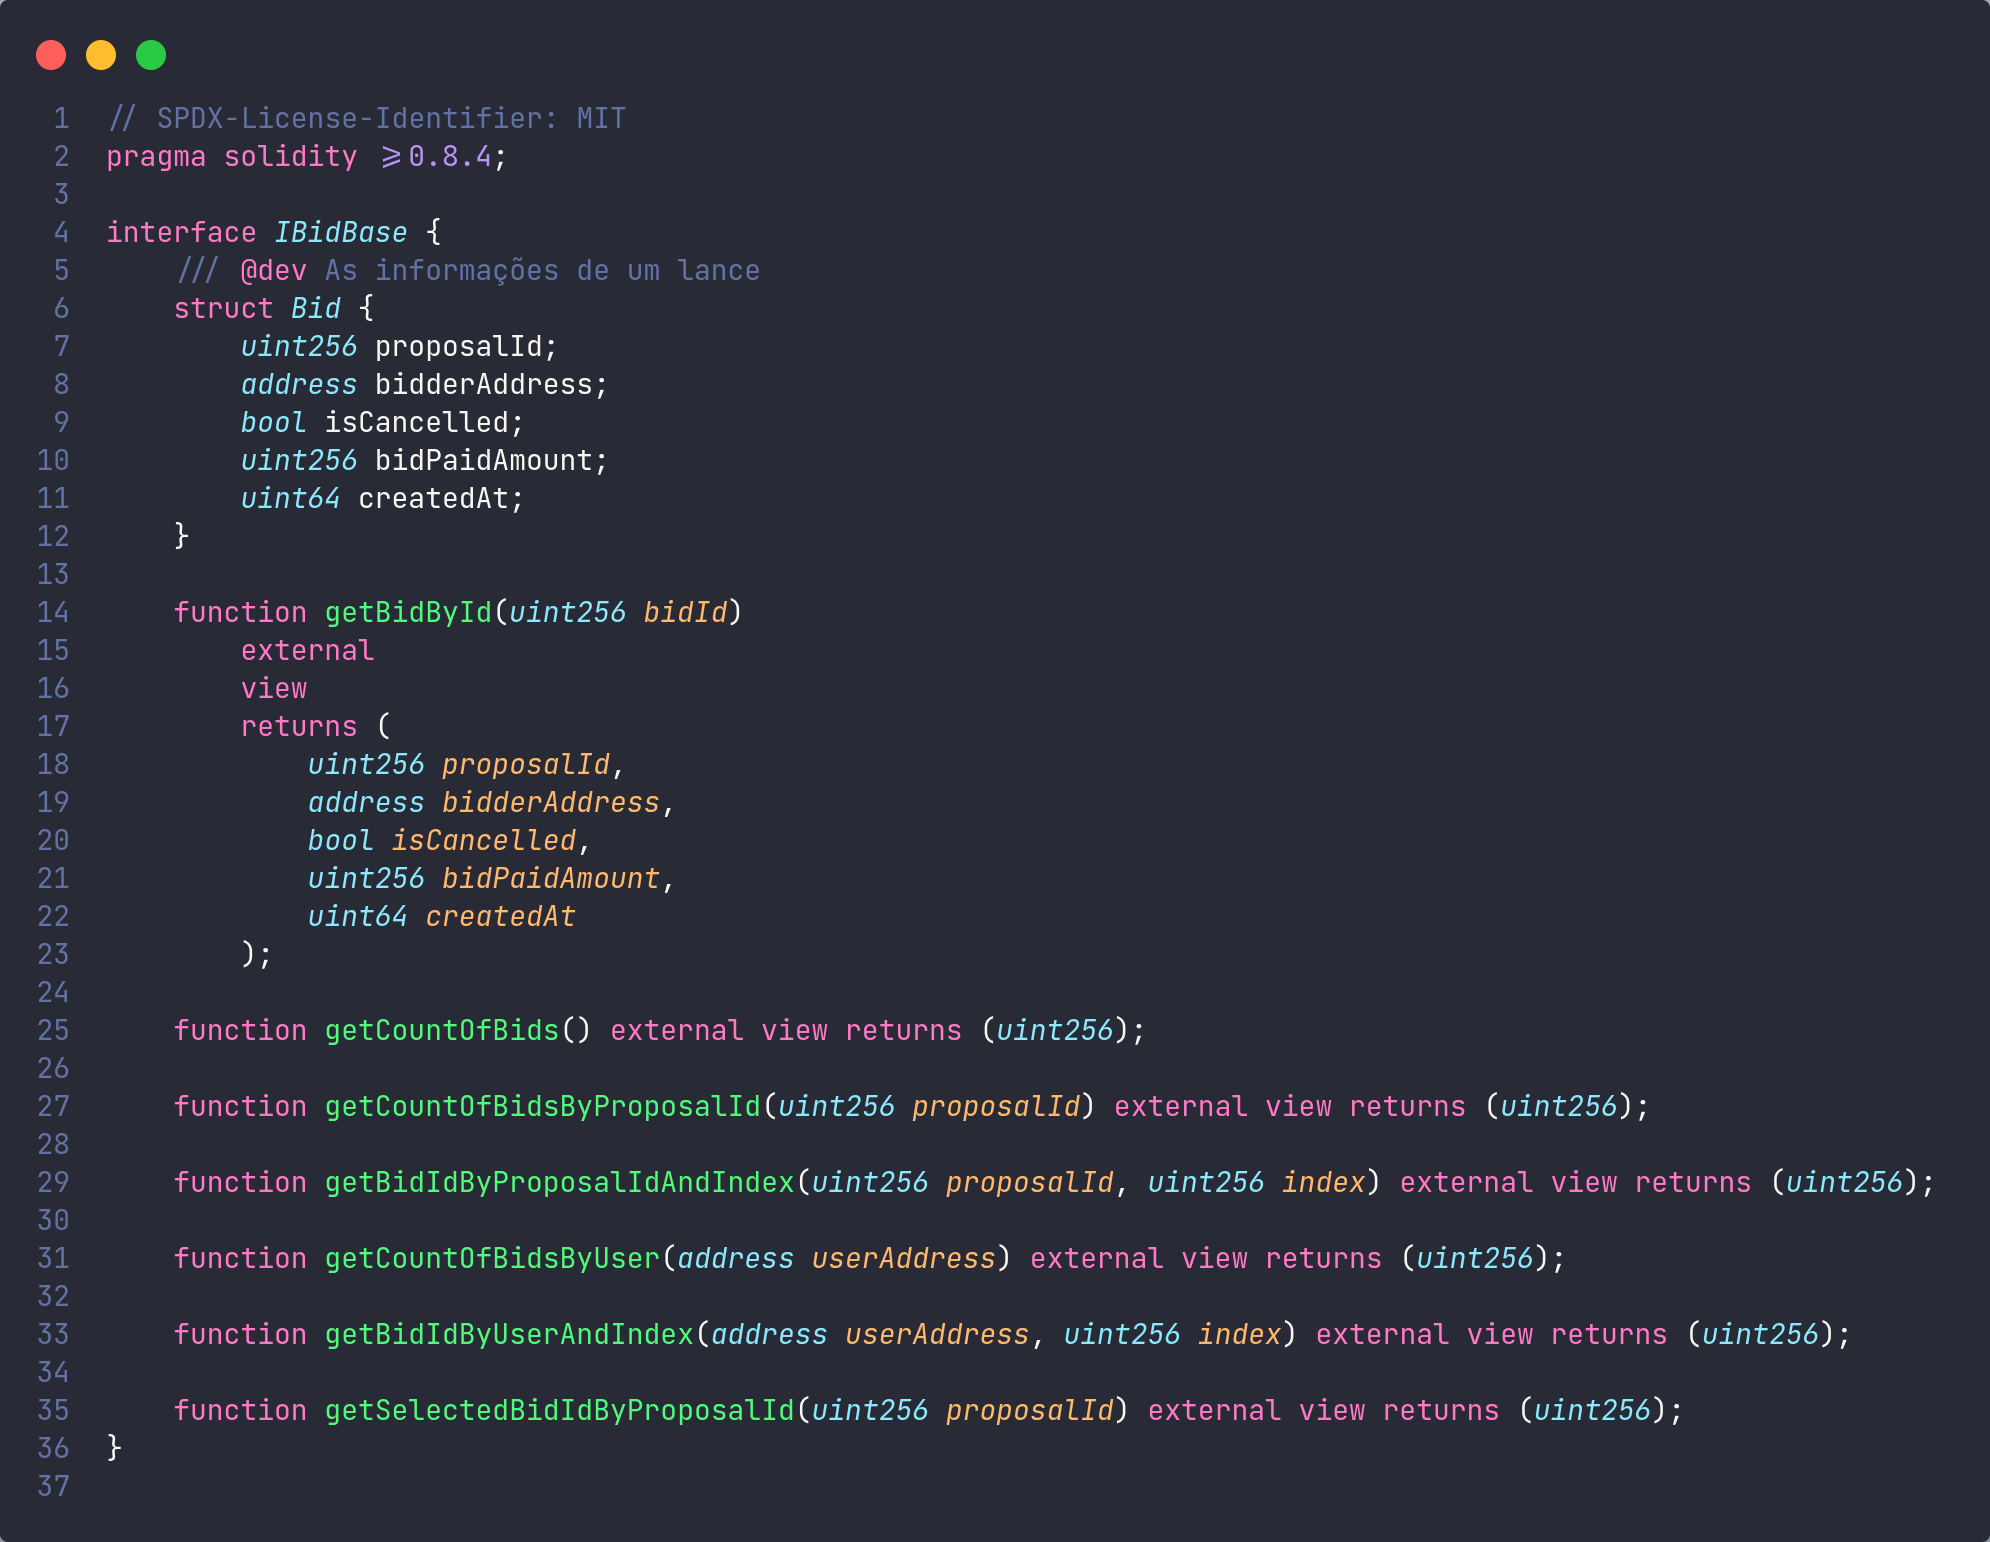
\includegraphics[width=420px]{src/images/contracts/bid_base.png}
  \subcaption{Fonte: Autor }
  \label{fig:bid_base_contract_fig}
\end{figure}

Pode-se observar que na figura \ref{fig:bid_base_contract_fig}, o contrato \textit{IBidBase} tem os métodos como \textit{getBidById} e \textit{getCountOfBids} para que o usuário possa listar todos os lances criados no contrato.

Além disso, há alguns métodos a mais que foram criados para que se possa integrar com as telas planejadas, como listar os lances de um usuário ou mesmo verificar qual lance foi selecionado para uma proposta.

E por fim, não foi criado uma interface para o contrato de \textit{BidProposal} porque esse contrato apenas expõe alguns métodos internos com a intenção de ser usado pelos métodos implementados das interfaces de \textit{IBidCore}.

Para ilustrar o propósito do contrato do \textit{BidProposal}, a figura \ref{fig:bid_proposal_fig} mostra o construtor do contrato e um dos métodos.

\begin{figure}[!h]
  \centering
  \caption{Contrato de Lances e Propostas}
  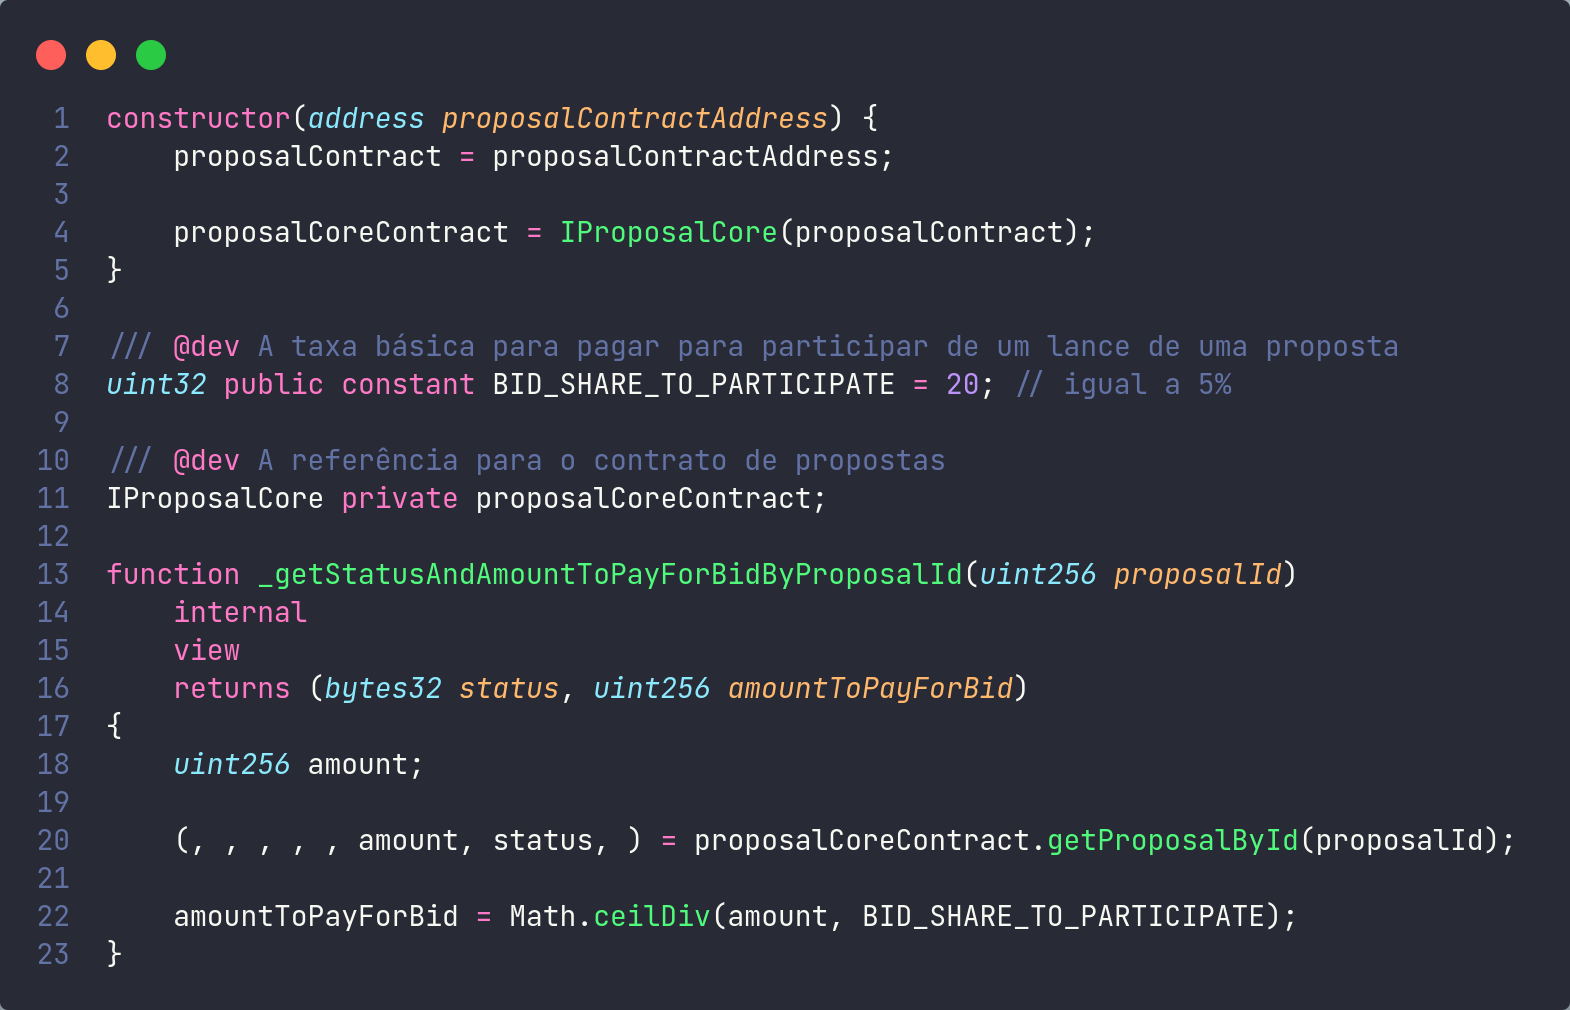
\includegraphics[width=420px]{src/images/contracts/bid_proposal.png}
  \subcaption{Fonte: Autor }
  \label{fig:bid_proposal_fig}
\end{figure}

Na linha 1 da figura \ref{fig:bid_proposal_fig}, o contrato irá receber o endereço do contrato de propostas, para que quando houver uma comunicação, seja assegurado que será do contrato de propostas correto. 

Há também uma constante chamada \textit{BID\_SHARE\_TO\_PARTICIPATE} que basicamente é usada para representar a porcentagem de quanto deve ser pago sobre o valor da proposta para que um lance seja criado. Essa constante é usada na linha 22 da figura \ref{fig:bid_proposal_fig}, no método que retorna o cálculo de quanto deve ser pago para criar um lance, assim como, saber o status da proposta.

\subsection{Disputas}

Para as disputas, foi divido em 2 interfaces e mais dois outros contratos que auxiliam a parte da comunicação com Lances e Propostas. As interfaces são \textit{IDisputeCore} e \textit{IDisputeBase}, junto dos contratos \textit{DisputeBid} e \textit{DisputeProposal}, responsáveis pela operações principais, operações básicas, comunicação com lances e comunicação com propostas, respectivamente.

A seguir, na figura \ref{fig:dispute_core_fig} será apresentado a interface \textit{IDisputeCore} que é usada para as operações principais.

\begin{figure}[!h]
  \centering
  \caption{Interface do contrato Core de Disputas}
  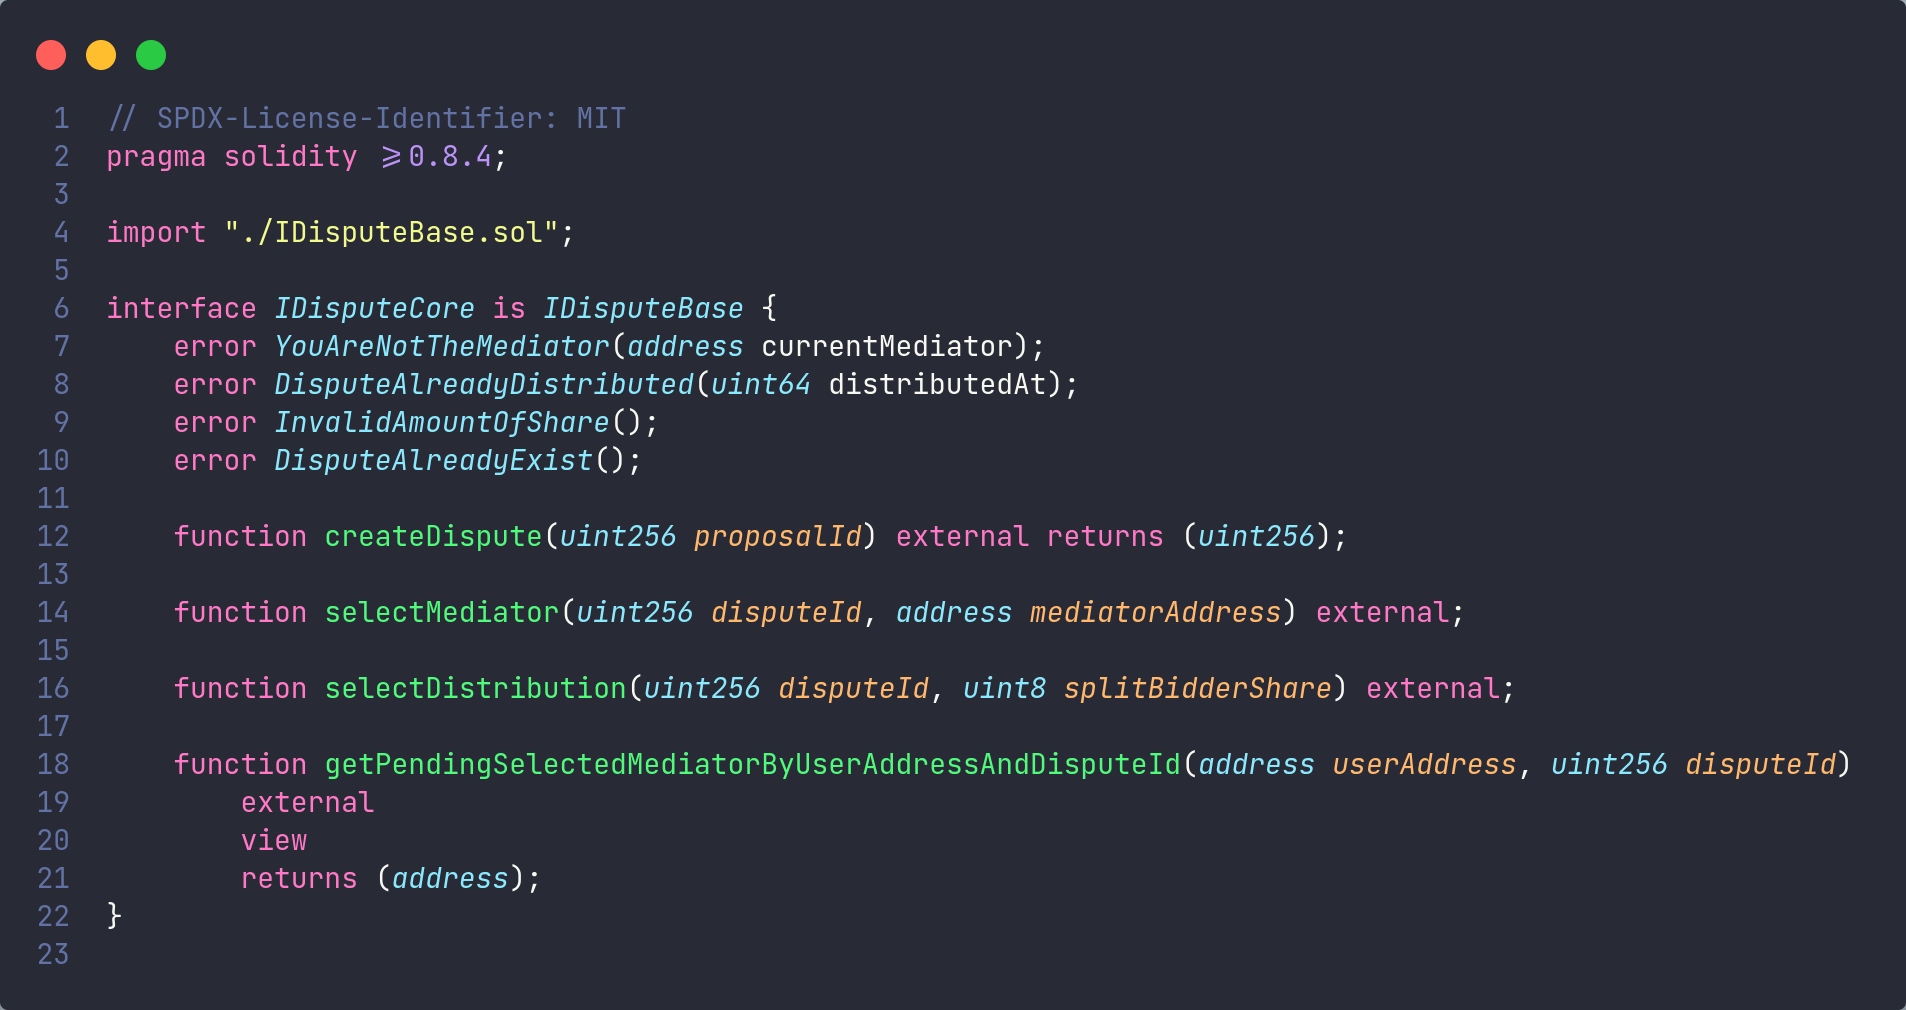
\includegraphics[width=420px]{src/images/contracts/dispute_core.png}
  \subcaption{Fonte: Autor }
  \label{fig:dispute_core_fig}
\end{figure}

Pode-se observar os métodos \textit{createDispute}, que é responsável pela criação de uma disputa, além de também notificar o contrato de proposta para atualizar o status da proposta.

Para as operações básicas, a figura \ref{fig:dispute_base_fig} mostra os métodos que são usados para listar as disputas, assim como mencionado anteriormente em propostas e lances, a combinação dos métodos de contar e buscar o item específico, no caso de disputa, \textit{getCountOfDisputes} e \textit{getDisputeById}.

\begin{figure}[!h]
  \centering
  \caption{Interface do contrato Base de Disputas}
  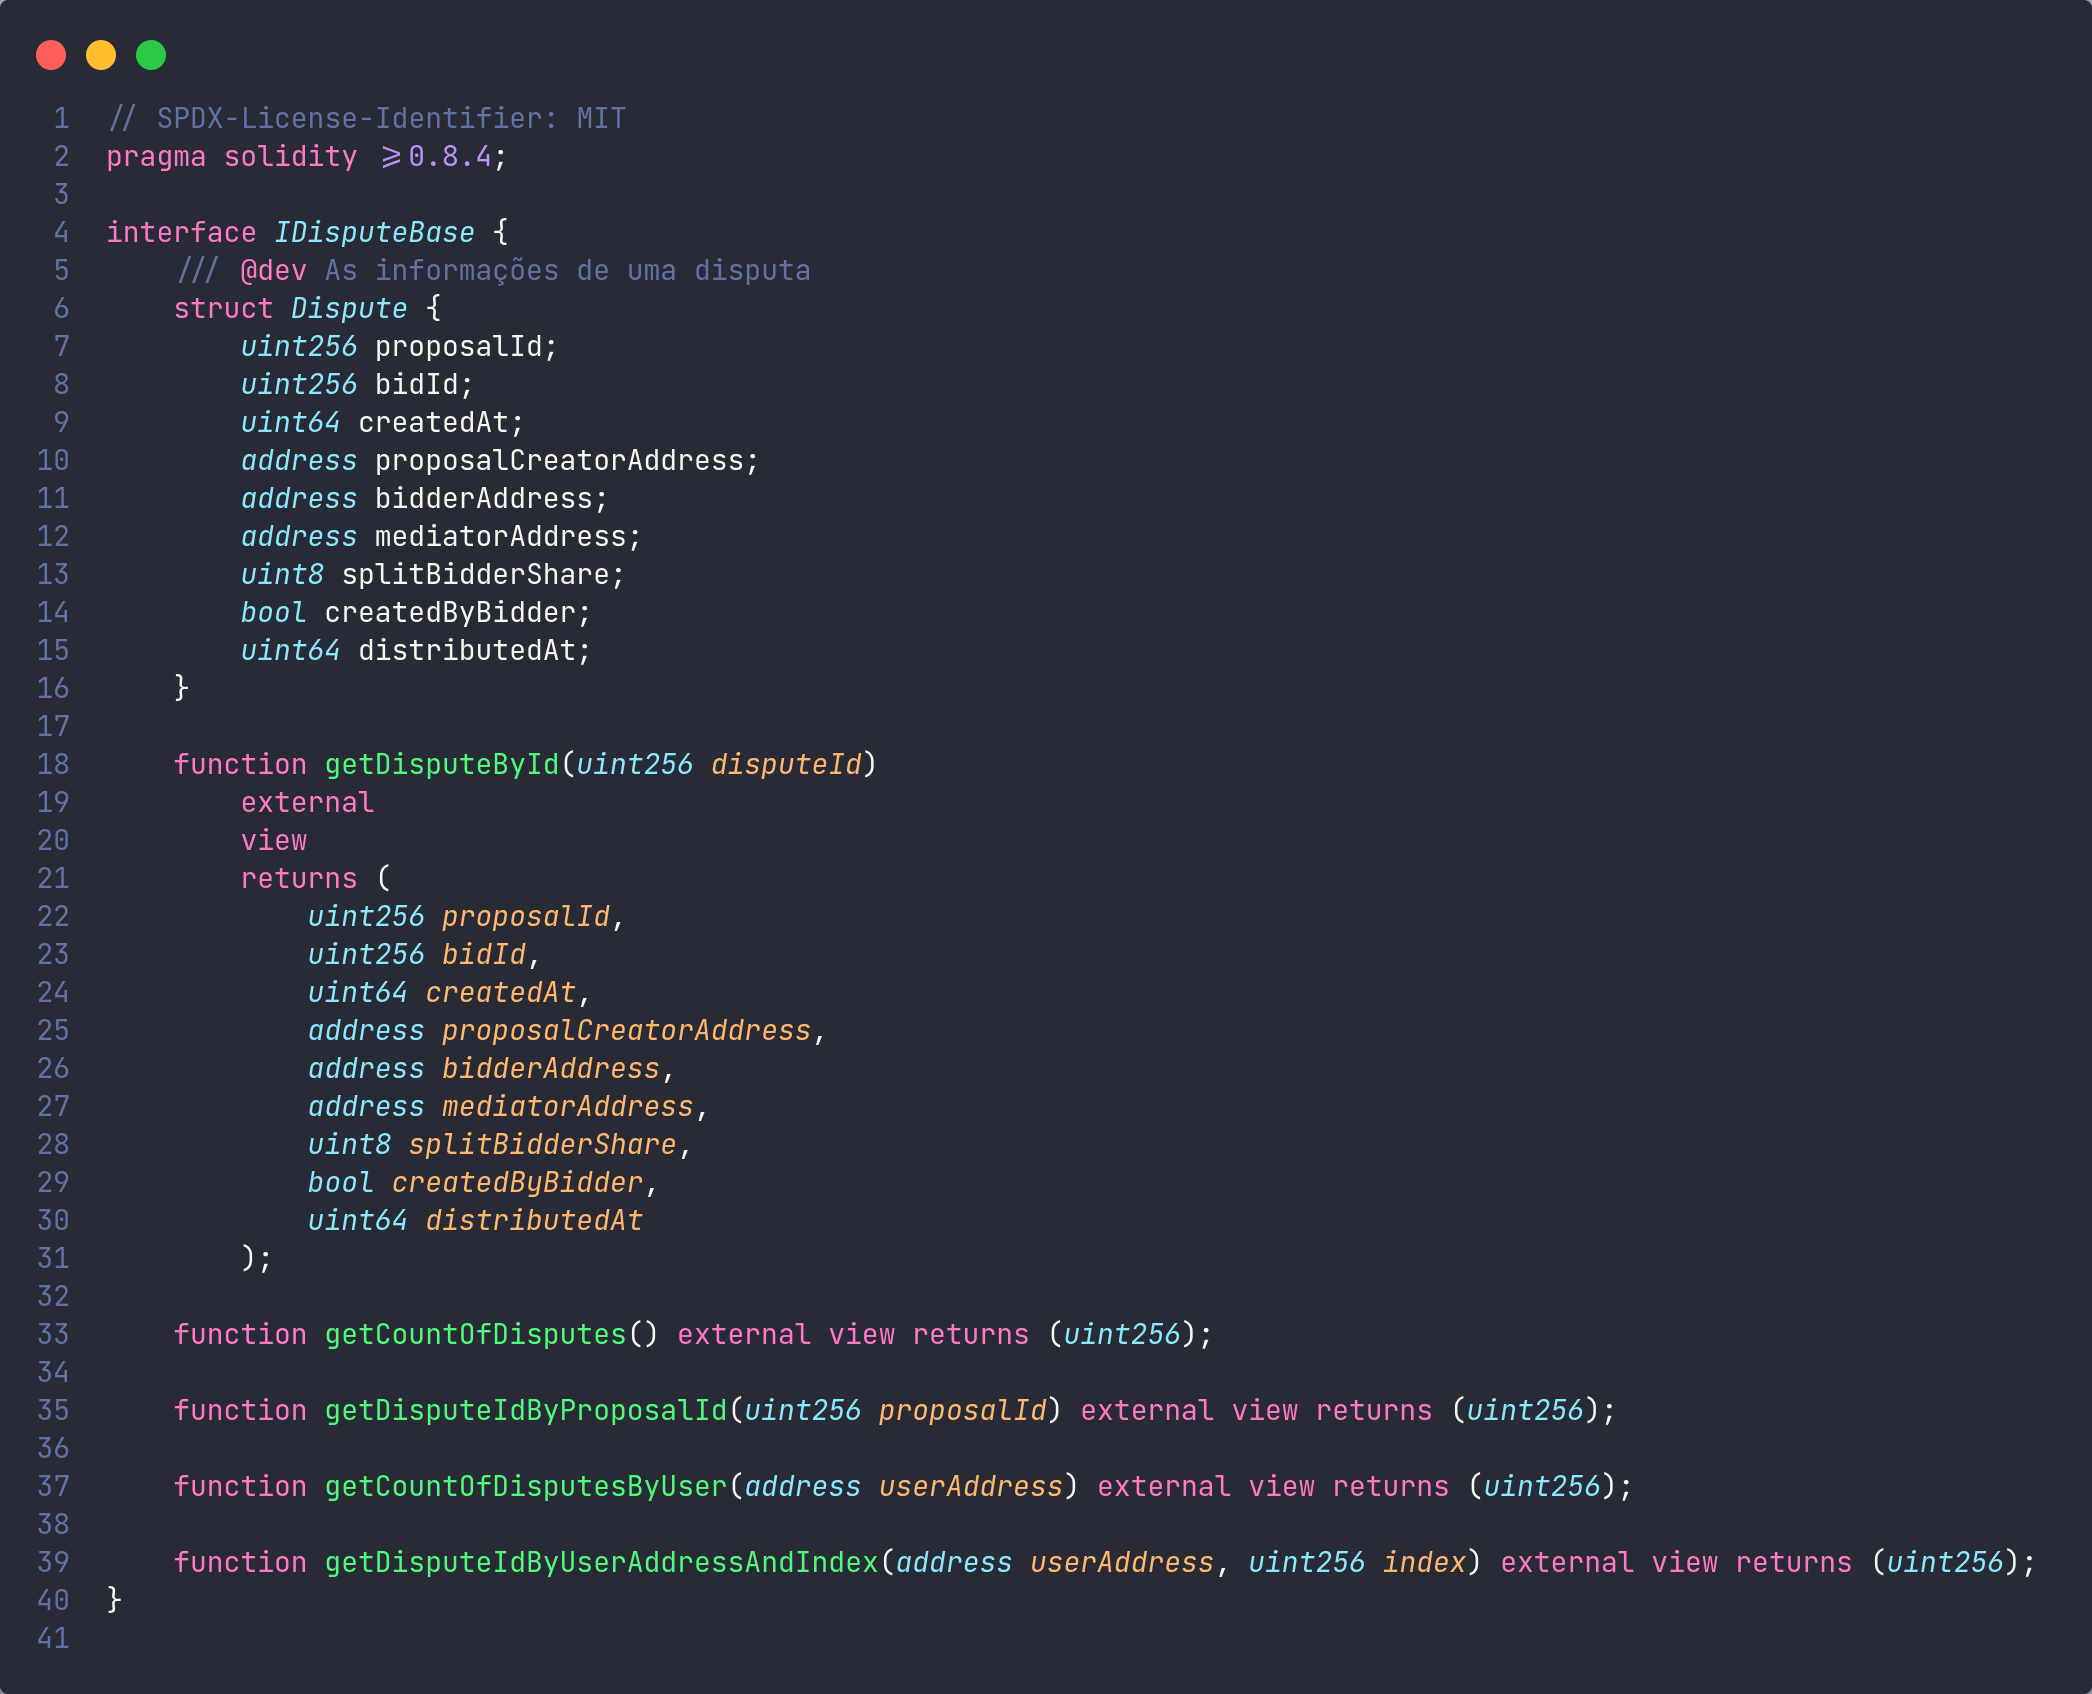
\includegraphics[width=360px]{src/images/contracts/dispute_base.png}
  \subcaption{Fonte: Autor }
  \label{fig:dispute_base_fig}
\end{figure}

Por fim, os dois contratos auxiliares, \textit{DisputeBid} e \textit{DisputeProposal} são exibidos nas figuras \ref{fig:dispute_bid_fig} e \ref{fig:dispute_proposal_fig}, respectivamente.

\begin{figure}[!h]
  \centering
  \caption{Contrato de Disputa e Lances}
  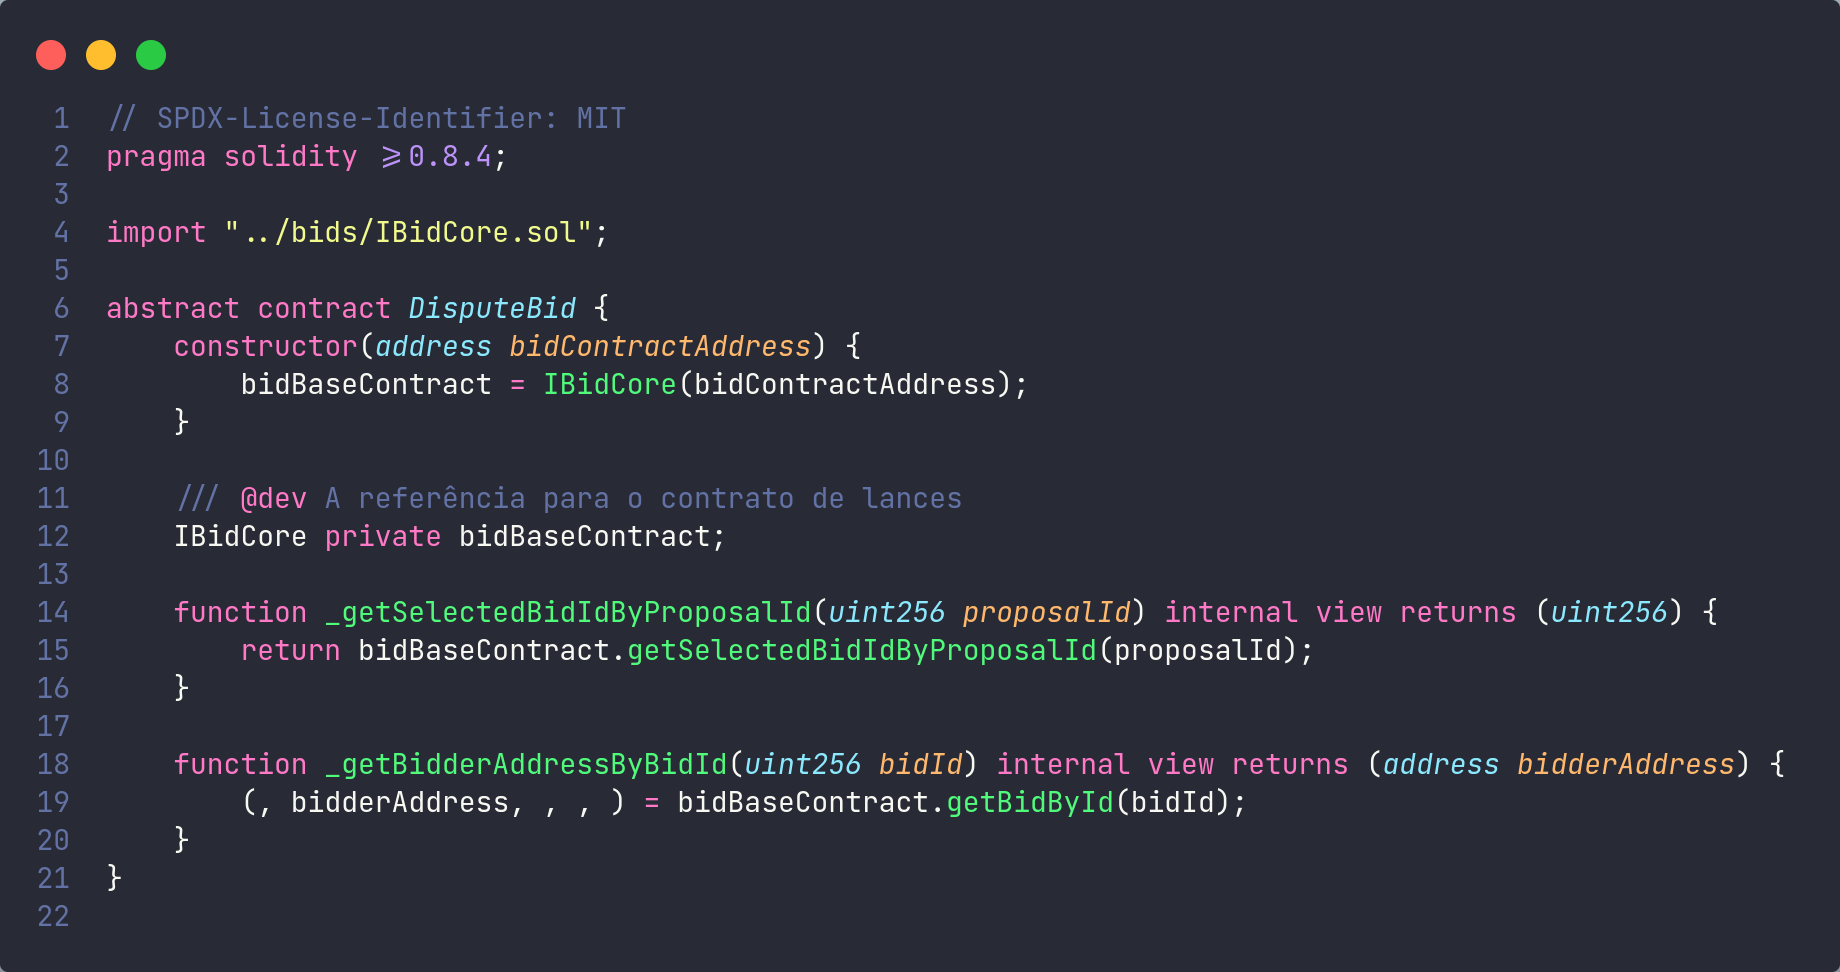
\includegraphics[width=400px]{src/images/contracts/dispute_bid.png}
  \subcaption{Fonte: Autor }
  \label{fig:dispute_bid_fig}
\end{figure}

\begin{figure}[!h]
  \centering
  \caption{Contrato de Disputa e Propostas}
  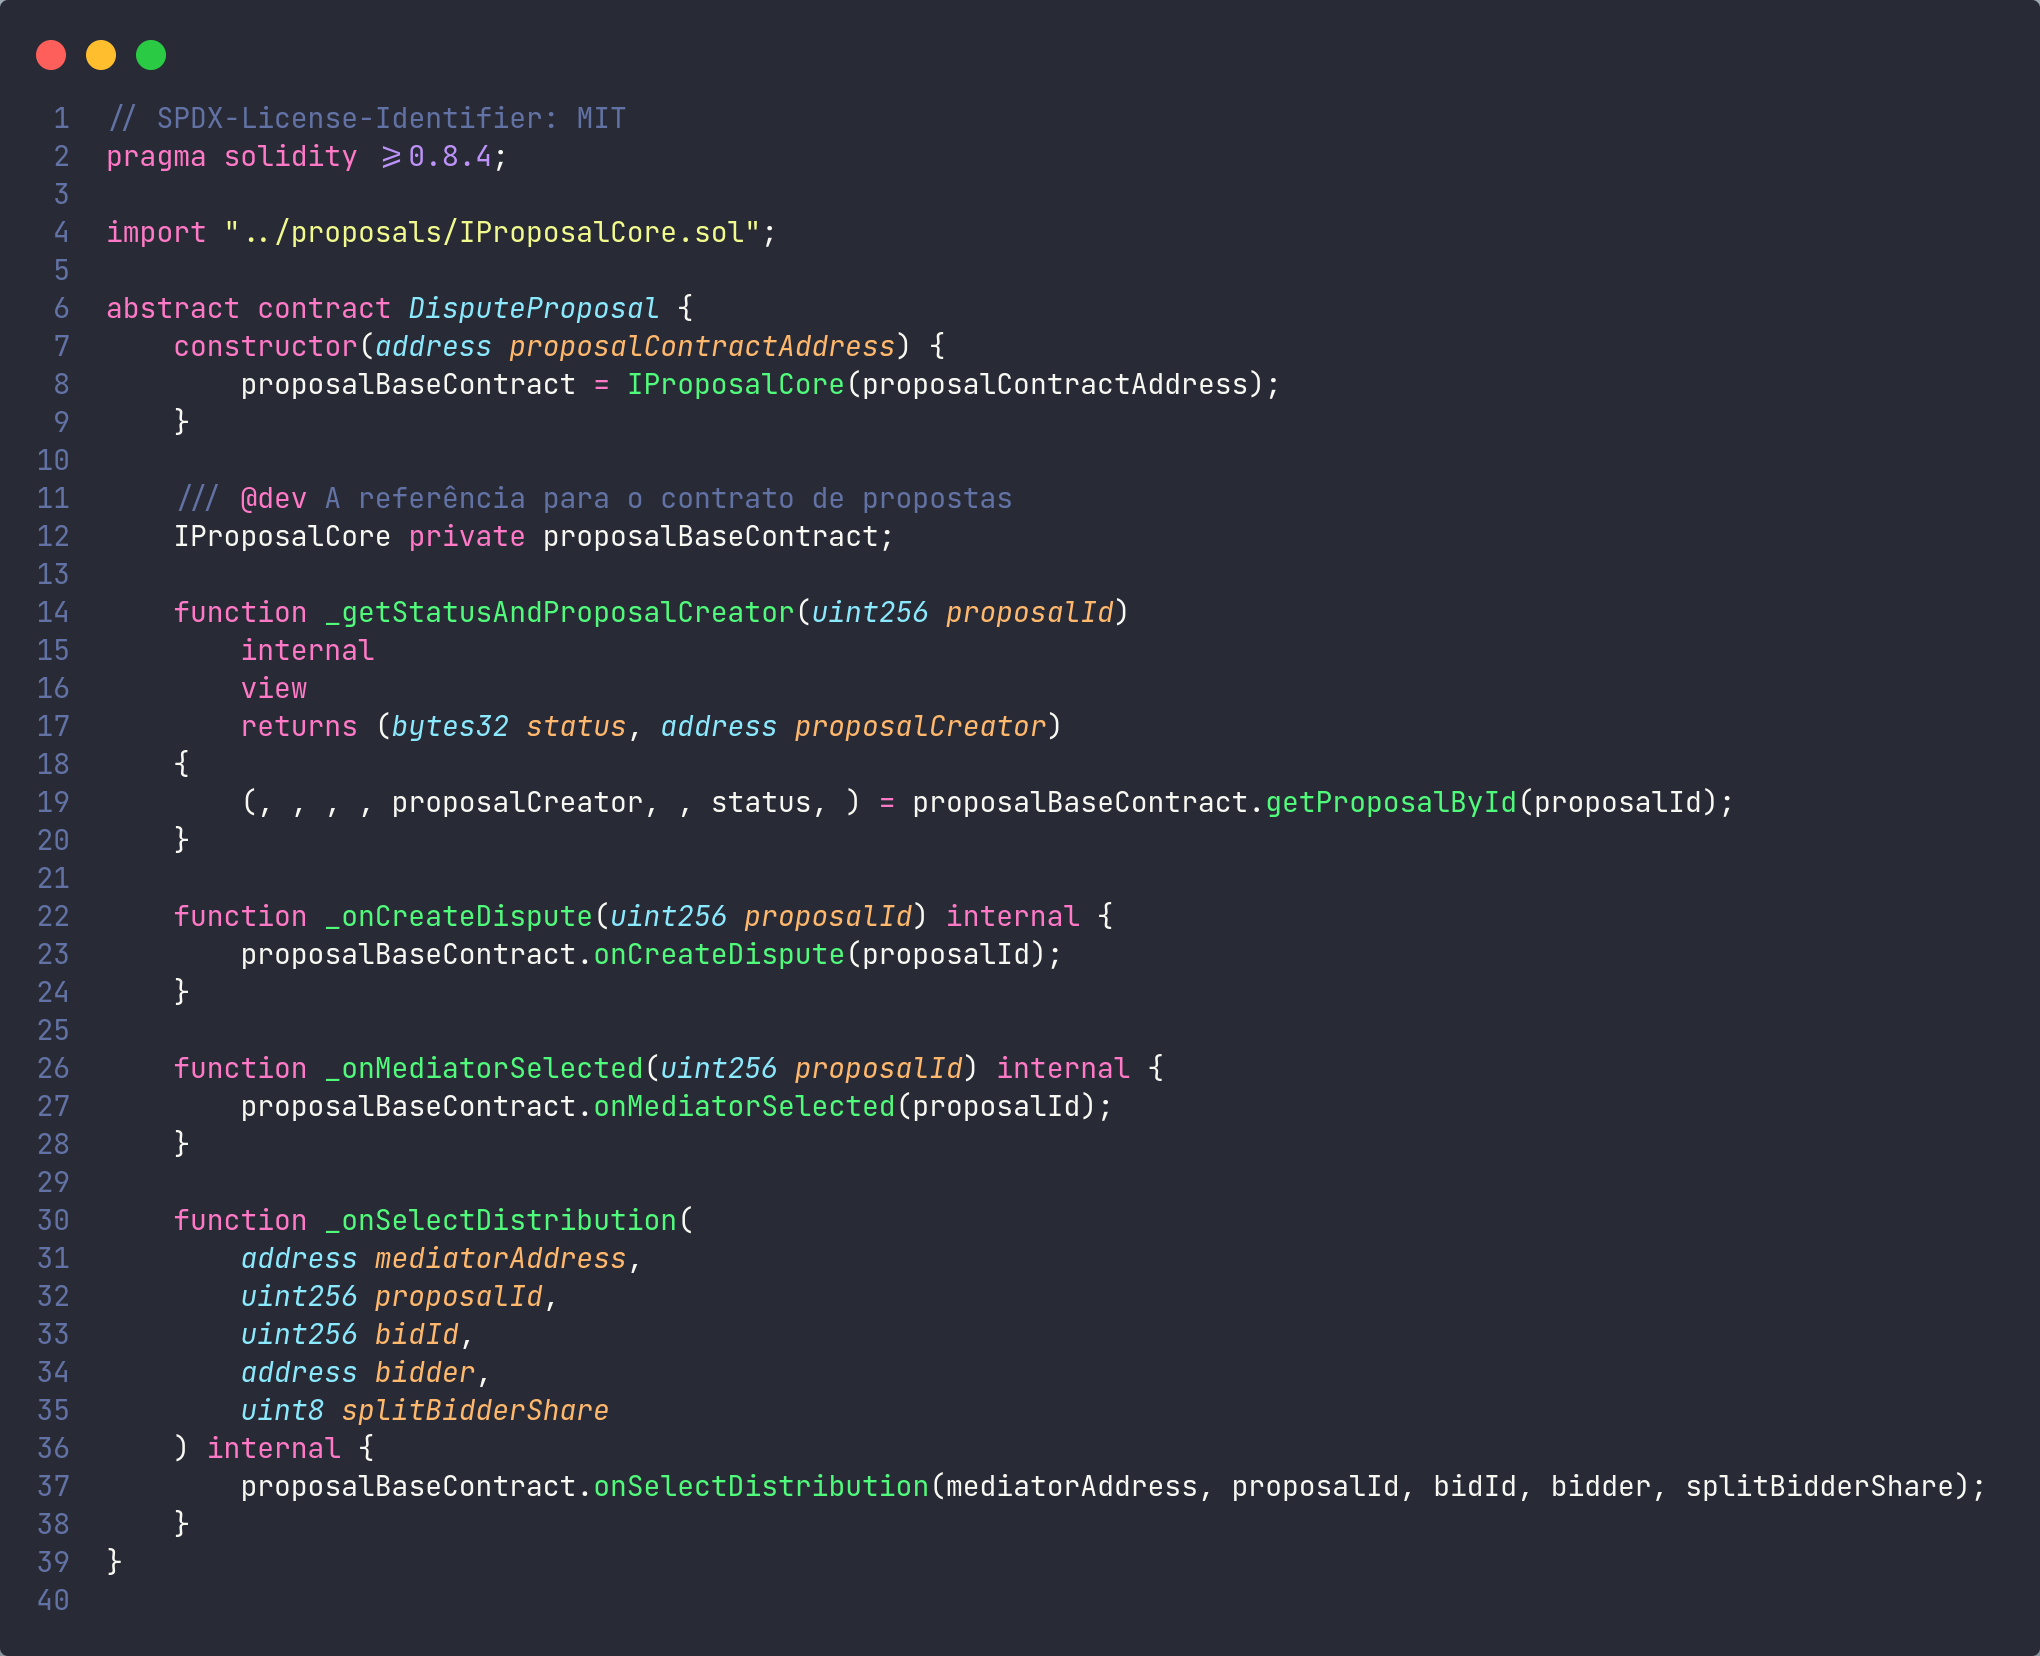
\includegraphics[width=350px]{src/images/contracts/dispute_proposal.png}
  \subcaption{Fonte: Autor }
  \label{fig:dispute_proposal_fig}
\end{figure}

Em ambos os contratos, as funções são principalmente para buscar o status da proposta, ou chamar os métodos de outros contratos para dizer que uma disputa foi criada, ou um mediador foi selecionado e até mesmo para transferir o valor dos contratos para quem o mediador preferiu.

Adentrando em mais especificidades dos contratos de disputa, é interessante analisar a implementação do método de \textit{selectDistribution} na figura \ref{fig:select_distribution_dispute_fig}, que é chamado pelo mediador para dividir os valores da proposta durante uma disputa.

\begin{figure}[!h]
  \centering
  \caption{Código do método de selectDistribution}
  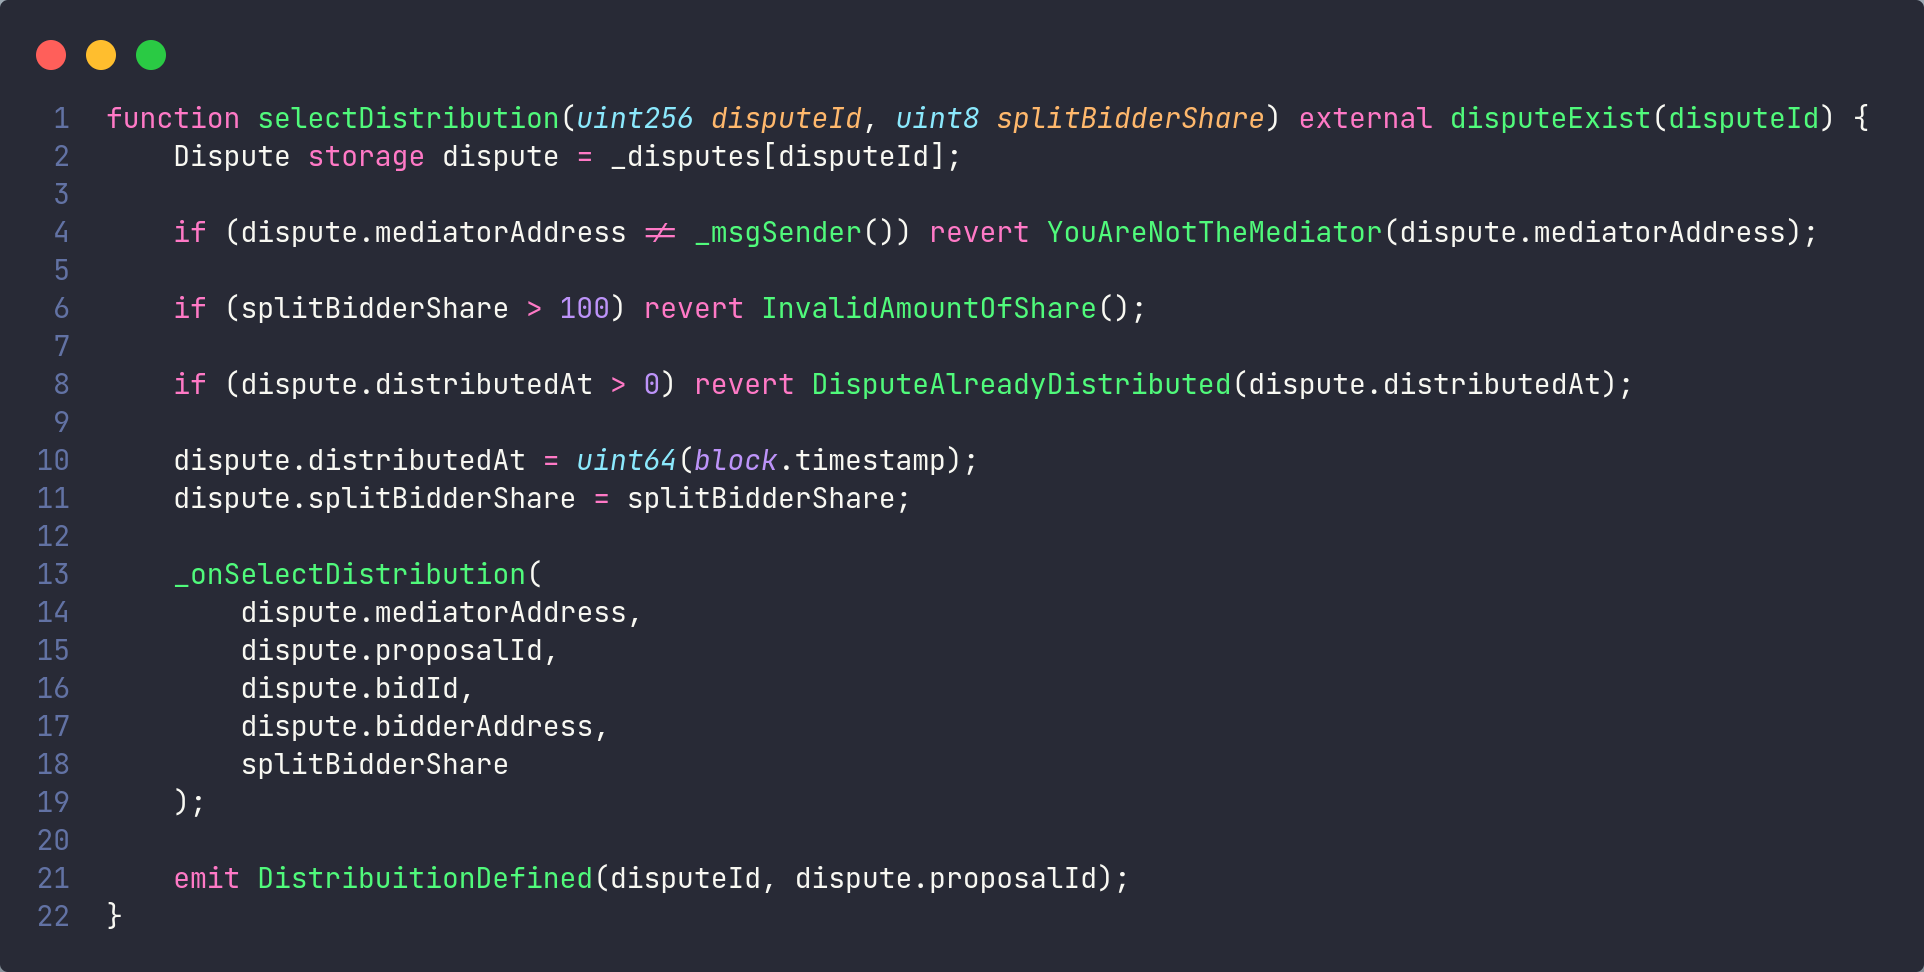
\includegraphics[width=400px]{src/images/contracts/select_distribution_dispute.png}
  \subcaption{Fonte: Autor }
  \label{fig:select_distribution_dispute_fig}
\end{figure}

Dentro desse método, ao analisar os quesitos de segurança, temos que na linha 8 da figura \ref{fig:select_distribution_dispute_fig} há uma validação para verificar se já foi distribuído os valores, e em seguida, na linha 10, é definido um valor para essa variável para que não permita que esse método seja chamado duas vezes.

Além disso, o método \textit{\_onSelectDistribution} é chamado para notificar os contratos de lance, que por sua vez, chama o contrato de propostas. A implementação no contrato de propostas pode ser observado na figura \ref{fig:on_select_distribution_proposal_fig}.

\begin{figure}[!h]
  \centering
  \caption{Código do método onSelectDistribution em propostas}
  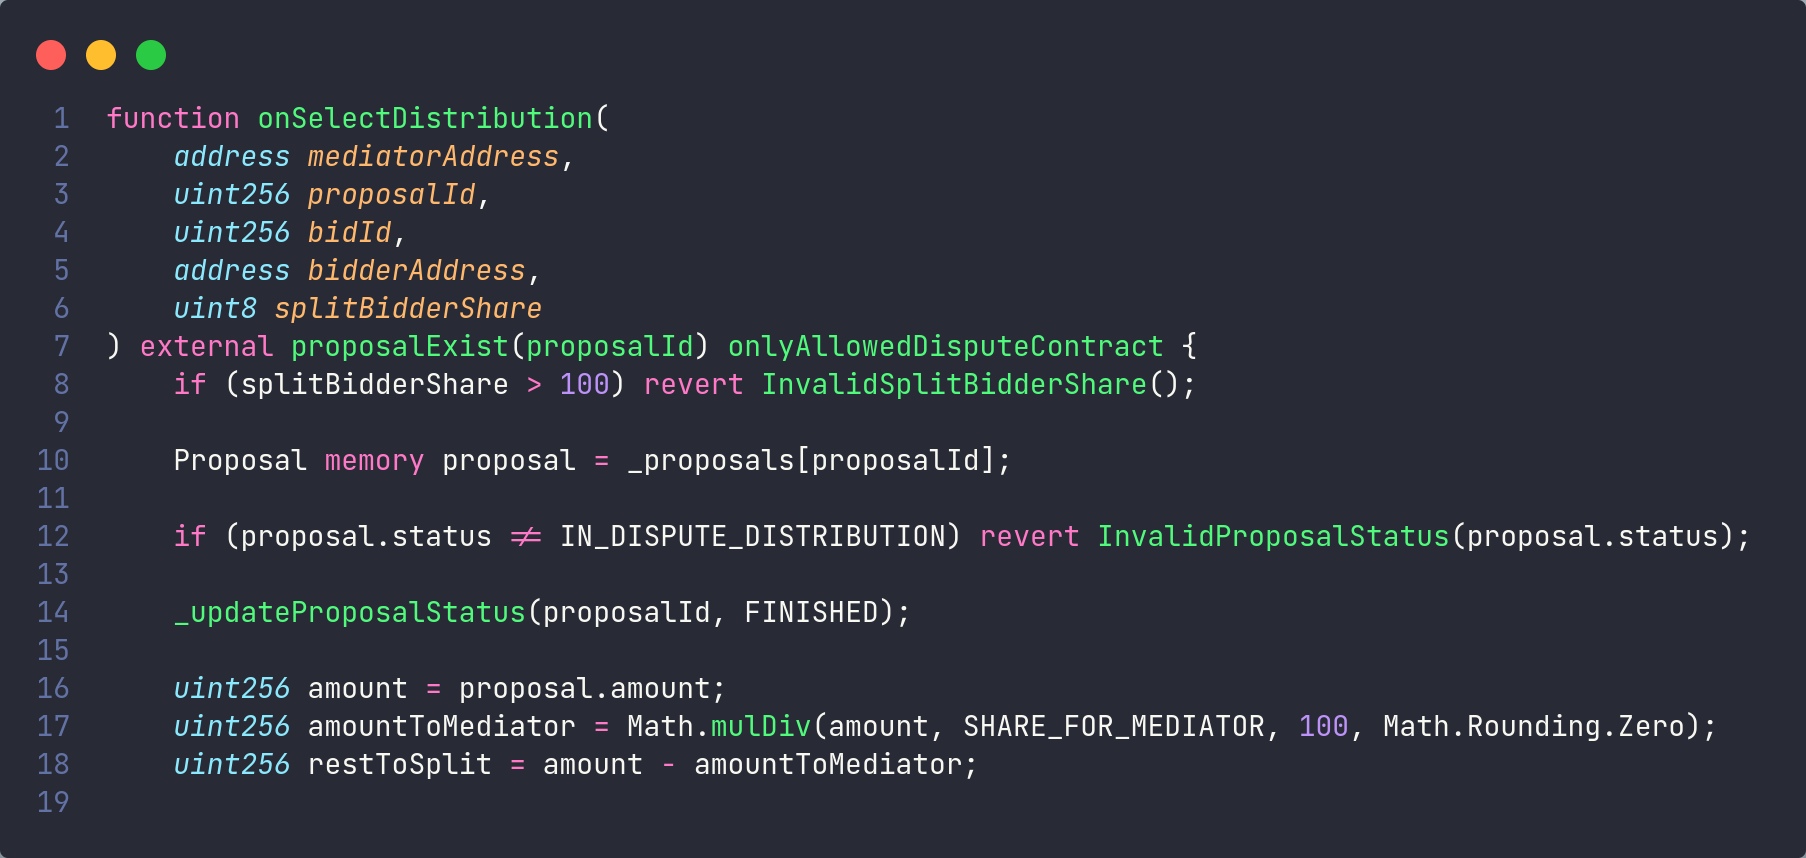
\includegraphics[width=320px]{src/images/contracts/on_select_distribution_proposal.png}
  \subcaption{Fonte: Autor }
  \label{fig:on_select_distribution_proposal_fig}
\end{figure}

Nas linhas 12 e 14 da figura \ref{fig:on_select_distribution_proposal_fig} há uma validação de segurança, e após isso, nas linhas 17 e 18 é calculado qual é o valor que será enviado para o mediador - 5\% do valor total da proposta - e o resto é divido de acordo com o que o mediador especificou. 

\subsection{Testes}

Para saber se o código escrito realmente fazia o que foi pretendido, foi escrito cerca de 71 testes no total para que fosse obtido uma cobertura de testes de 100\%. 
% A seguir, as figuras (\ref{fig:tests_proposal_fig}), (\ref{fig:tests_bid_fig}) e (\ref{fig:tests_dispute_fig}) representam, respectivamente, os testes dos contratos de Proposta, Lances e Disputa.
A seguir, na figura \ref{fig:tests_proposal_fig} é mostrado os testes criados para o contrato de proposta.

\begin{figure}[!h]
  \centering
  \caption{Testes do contrato de proposta}
  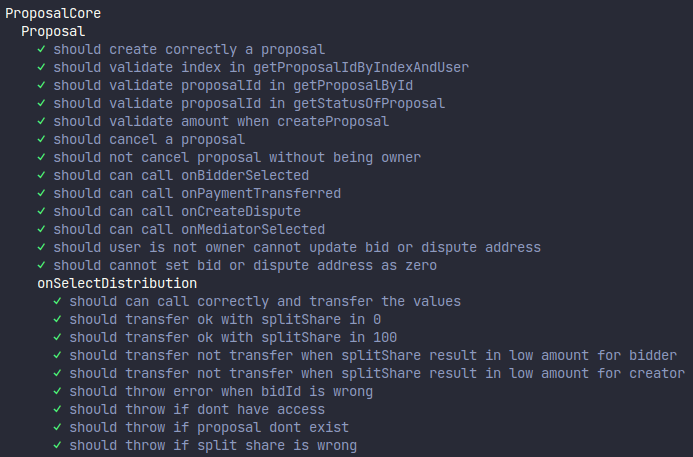
\includegraphics[width=400px]{src/images/contracts/tests_proposal.png}
  \subcaption{Fonte: Autor }
  \label{fig:tests_proposal_fig}
\end{figure}

É importante notar que foi criado sub-categorias nos testes para os métodos que realizam uma operação dentro do contrato de proposta, e para os métodos de visualização, os testes para eles são feitos durante os testes principais.

Após os testes de propostas, há os testes do contrato de disputa, que pode ser observado na figura \ref{fig:tests_bid_fig}.

\begin{figure}[!h]
  \centering
  \caption{Testes do contrato de lances}
  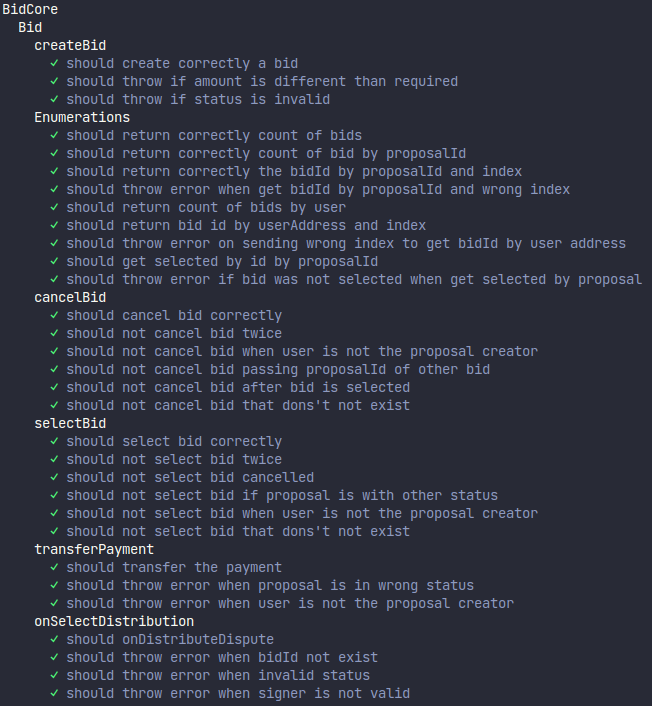
\includegraphics[width=320px]{src/images/contracts/tests_bid.png}
  \subcaption{Fonte: Autor }
  \label{fig:tests_bid_fig}
\end{figure}

E assim como no contrato de proposta, o foco dos testes do contrato de lances é testar os métodos que modificam o estado da \textit{Blockchain}. Além disso, o contrato de Lances é o que possui a maior quantidade de testes devido a quantidade a complexidade de suas operações.

E por fim, na figura \ref{fig:tests_dispute_fig} pode-se observar os testes escritos para o contrato de disputa, no qual o foco está em testar os métodos principais de criação de disputa, selecionar mediador e realizar a distribuição dos valores da proposta.

\begin{figure}[!h]
  \centering
  \caption{Testes do contrato de disputas}
  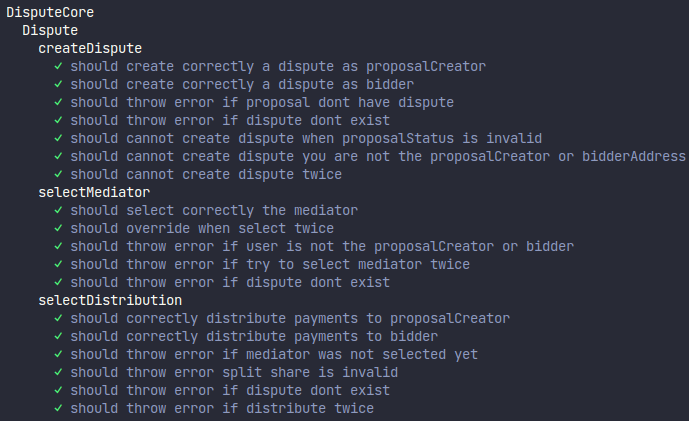
\includegraphics[width=320px]{src/images/contracts/tests_dispute.png}
  \subcaption{Fonte: Autor }
  \label{fig:tests_dispute_fig}
\end{figure}

Dessa forma, com os testes feitos, pode-se ter uma segurança maior que, o que foi proposto no desenvolvimento, será executado corretamente. Além disso, na figura \ref{fig:tests_coverage_fig}, há cobertura dos testes desenvolvidos.

\begin{figure}[!h]
  \centering
  \caption{Testes do contrato de proposta}
  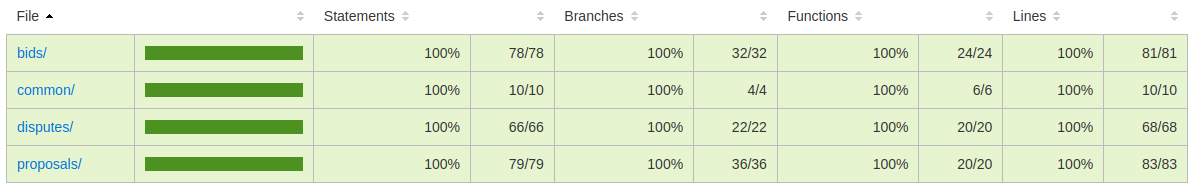
\includegraphics[width=450px]{src/images/contracts/tests_coverage.png}
  \subcaption{Fonte: Autor }
  \label{fig:tests_coverage_fig}
\end{figure}

E conforme pode ser observado na figura \ref{fig:tests_coverage_fig}, tanto as linhas quanto as \textit{branches} estão em 100\%, que significa todas as ramificações e caminhos possíveis no código estão com uma cobertura completa.

\subsection{Consumo de \texit{Gas}}

Um fator importante para a viabilidade da plataforma é saber o quanto de \textit{Gas} cada operação que modifica o estado da \textit{Blockchain} está consumindo. A seguir, é mostrado na tabela \ref{tab:report_gas} o consumo médio de cada método por contrato.

\begin{table}[!h]
\centering
\caption{Consumo de Gas por método}
\label{tab:report_gas}
\begin{tabular}{@{}lll@{}}
\toprule
Contrato & Método    & Média (gas) \\ \midrule
Proposta & cancelProposal & 55416 \\
Proposta & createProposal & 301054 \\
Proposta & onBidderSelected & 50589 \\
Proposta & onCreateDispute & 50512 \\
Proposta & onMediatorSelected & 50457 \\
Proposta & onPaymentTransferred & 60541 \\
Proposta & onSelectDistribution & 108538 \\
Proposta & setBidContractAddress & 42251 \\
Proposta & setDisputeContractAddress & 31531 \\
Lance & cancelBid & 44540 \\
Lance & createBid & 296738 \\
Lance & onSelectDistribution & 72834 \\
Lance & selectBid & 99942 \\
Lance & transferPayment & 91653 \\
Dispute & createDispute & 373572 \\
Dispute & selectDistribution & 126345 \\
Dispute & selectMediator & 73402 \\ \bottomrule
\end{tabular}
\begin{tablenotes}
  \small
  \item Fonte: Autor
\end{tablenotes}
\end{table}

Além do consumo por método, foi medido também o consumo de \textit{Gas} para hospedar o contrato na rede \textit{Blockchain}, esse consumo é mostrado na tabela \ref{tab:report_gas_contract}.

\begin{table}[!h]
\centering
\caption{Consumo de Gas por contrato}
\label{tab:report_gas_contract}
\begin{tabular}{@{}lll@{}}
\toprule
Contrato    & Média (gas) \\ \midrule
Proposta  & 1372426 \\
Lance     & 1236650 \\
Disputa   & 2495562 \\ \bottomrule
\end{tabular}
\begin{tablenotes}
  \small
  \item Fonte: Autor
\end{tablenotes}
\end{table}

O consumo do contrato é calculado pela quantidade de código - também chamado por \textit{bytecode} - resultante da compilação do contrato. Para entender melhor a quantidade de \textit{Gas}, veja a tabela \ref{tab:report_contract_size} para verificar o tamanho do contrato em bytes.

\begin{table}[!h]
\centering
\caption{Tamanho em bytes por contrato}
\label{tab:report_contract_size}
\begin{tabular}{@{}lll@{}}
\toprule
Contrato  & Tamanho (KiB) \\ \midrule
Proposta  & 10,931 \\
Lance     & 5,641 \\
Disputa   & 5,021 \\ \bottomrule
\end{tabular}
\begin{tablenotes}
  \small
  \item Fonte: Autor
\end{tablenotes}
\end{table}

Para ter uma comparação, o tamanho máximo permitido para um contrato, segundo EIP 170, é definido como 24KiB. Até pode parecer bastante mas dependendo de que tipo de operação você escolhe e como organizar os contratos, o tamanho pode realmente se aproximar facilmente do limite. E ao atingir esse limite, a única escolha é dividir o contrato ou buscar otimizar o contrato.

Por fim, para dar contexto ao consumo de \textit{Gas}, é necessário calcular a taxa de cada operação através da taxa base em \textit{Gwei}, que é a menor unidade da moeda de um \textit{Ether} ou \textit{Matic}, multiplicado pelo \textit{Gas} usado. Dessa forma, na tabela \ref{tab:report_gwei_price}, é mostrado a taxa base em \textit{Gwei} na rede no qual foi feito a hospedagem dos contratos (\textit{Polygon}), assim como, na rede \textit{Ethereum} para ter uma comparação, por data.

\begin{table}[!h]
\centering
\caption{Taxa base na Ethereum e Polygon}
\label{tab:report_gwei_price}
\begin{tabular}{@{}lll@{}}
\toprule
Data  & Ethereum (Gwei) & Polygon (Gwei) \\ \midrule
01/09/2019  & 14,73 & Sem dados \\ 
01/05/2022  & 60,05 & 90,26 \\ 
01/10/2022  & 11,41 & 154,21 \\ \bottomrule
\end{tabular}
\begin{tablenotes}
  \small
  \item Fonte: \cite{ethereum_gwei_price} e \cite{polygon_gwei_price}
\end{tablenotes}
\end{table}

Com a taxa base, é necessário entender quanto custa cada \textit{Gwei} consumido, para que, ao ter o valor multiplicado, seja possível obter o valor de cada operação em R\$. Dessa forma, na tabela \ref{tab:report_gwei_to_real} é mostrado o preço de cada \texit{Gwei} em reais.

\begin{table}[!h]
\centering
\caption{Preço de um Gwei na Ethereum e Polygon}
\label{tab:report_gwei_to_real}
\begin{tabular}{@{}lll@{}}
\toprule
Data  & Ethereum (R\$) & Polygon (R\$) \\ \midrule
01/09/2019  & 1424,87 & Sem dados \\ 
01/05/2022  & 14551,91 & 5,66 \\ 
01/10/2022  & 6772,92 & 3,98 \\ \bottomrule
\end{tabular}
\begin{tablenotes}
  \small
  \item Fonte: \cite{ethereum_price_2019}, \cite{ethereum_price_2022} e \cite{ethereum_price_10_2022} convertido usando 5,16370 REAL/USD corrigido pela inflação do período. \cite{inflation_calculator}.
\end{tablenotes}
\end{table}

Pode-se observar, na tabela \ref{tab:report_gwei_to_real}, que em 2019 não há dados para a \textit{Polygon}, isso acontece porque ela só foi lançada em 2020.

Por fim, usando a referência que 1 ether que é igual a \(10^9\) Gwei, usando os custos da taxa e o preço de cada moeda, o preço da taxa de cada operação na rede \texit{Ethereum} foi calculado e representado na tabela \ref{tab:report_prices_per_method_ethereum}, e para a rede Polygon na tabela \ref{tab:report_prices_per_method_polygon}.

\begin{table}[!h]
\centering
\caption{Preço da taxa de cada operação na Ethereum}
\label{tab:report_prices_per_method_ethereum}
\begin{tabular}{@{}llll@{}}
\toprule
Método & 01/09/2019 (R\$) & 01/05/2022 (R\$) & 01/10/2022 (R\$) \\ \midrule
cancelProposal & 1,16 & 48,42 & 4,28 \\
createProposal & 6,32 & 263,07 & 23,27 \\
onBidderSelected & 1,06 & 44,21 & 3,91 \\
onCreateDispute & 1,06 & 44,14 & 3,90 \\
onMediatorSelected & 1,06 & 44,09 & 3,90 \\
onPaymentTransferred & 1,27 & 52,90 & 4,68 \\
onSelectDistribution & 2,28 & 94,85 & 8,39 \\
setBidContractAddress & 0,89 & 36,92 & 3,27 \\
setDisputeContractAddress & 0,66 & 27,55 & 2,44 \\
cancelBid & 0,93 & 38,92 & 3,44 \\
createBid & 6,23 & 259,30 & 22,93 \\
onSelectDistribution & 1,53 & 63,65 & 5,63 \\
selectBid & 2,10 & 87,33 & 7,72 \\
transferPayment & 1,92 & 80,09 & 7,08 \\
createDispute & 7,84 & 326,44 & 28,87 \\
selectDistribution & 2,65 & 110,41 & 9,76 \\
selectMediator & 1,54 & 64,14 & 5,67 \\ \bottomrule
\end{tabular}
\begin{tablenotes}
  \small
  \item Fonte: Autor
\end{tablenotes}
\end{table}

\begin{table}[!h]
\centering
\caption{Preço da taxa de cada operação na Polygon}
\label{tab:report_prices_per_method_polygon}
\begin{tabular}{@{}lll@{}}
\toprule
Método & 01/05/2022 (R\$) & 01/10/2022 (R\$) \\ \midrule
cancelProposal & 0,03 & 0,03 \\
createProposal & 0,15 & 0,18 \\
onBidderSelected & 0,03 & 0,03 \\
onCreateDispute & 0,03 & 0,03 \\
onMediatorSelected & 0,03 & 0,03 \\
onPaymentTransferred & 0,03 & 0,04 \\
onSelectDistribution & 0,06 & 0,07 \\
setBidContractAddress & 0,02 & 0,03 \\
setDisputeContractAddress & 0,02 & 0,02 \\
cancelBid & 0,02 & 0,03 \\
createBid & 0,15 & 0,18 \\
onSelectDistribution & 0,04 & 0,04 \\
selectBid & 0,05 & 0,06 \\
transferPayment & 0,05 & 0,06 \\
createDispute & 0,19 & 0,23 \\
selectDistribution & 0,06 & 0,08 \\
selectMediator & 0,04 & 0,05 \\ \bottomrule
\end{tabular}
\begin{tablenotes}
  \small
  \item Fonte: Autor
\end{tablenotes}
\end{table}